\chapter{Experimental Evaluation} \label{chap:results}
In this chapter the methods introduced in the previous sections are evaluated and results are presented. In \cref{sec:verification_of_nn} the implemented classification framework called \textit{kitt\_nn} (see \cref{chap:kitt_nn} and details in \cref{sec:implementation_of_nn}) is verified by comparing to a publicly provided framework. The results of the developed pruning algorithm are shown in \cref{sec:pruning_algorithm_results}. Then, the overall terrain classification process is gradually evaluated in \cref{sec:terrain_processing_results}.

\section{Verification of the Network Implementation} \label{sec:verification_of_nn}
Classification performance of the implemented method \textit{kitt\_nn} is compared to a \textit{Scikit-neuralnetwork} classifier (\citep{misc:sknn}) presented in \cref{ssec:sknn}. The evaluation is performed on two datasets introduced in \cref{ssec:testing_datasets}.

The following \cref{fig:kitt_verify_acc} shows the progress of classification accuracy within learning epochs. For each dataset/framework combination, $ 10 $ observations were performed and mean values with standard deviation ranges are shown.

\begin{figure}[H]
  \centering
  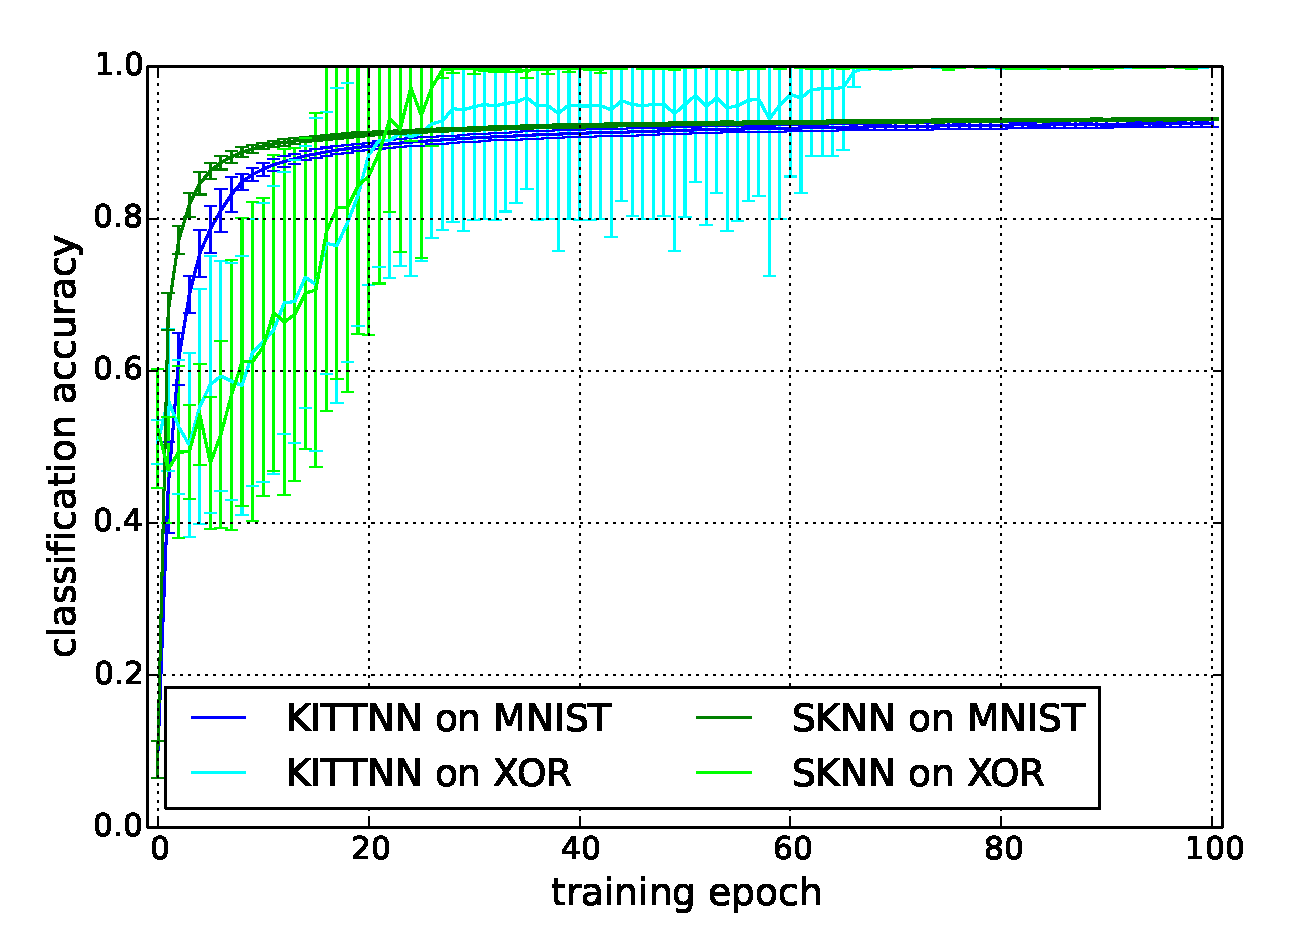
\includegraphics[width=0.8\textwidth]{kitt_verify_acc}
  \caption{Learning process compared to another framework (Scikit-neuralnetwork (sknn): \citep{misc:sknn}).}
  \label{fig:kitt_verify_acc}
\end{figure}

Regarding the XOR dataset, both nets start with the accuracy of about $ 0.5 $, as it has $ 2 $ classes and, naturally, with accuracy of about $ 0.1 $ for the $ 10 $ classes of the MNIST dataset. Individual observations differ more to each other (see the standard deviation in \cref{fig:kitt_verify_acc}) for XOR, as there are a lot less training samples compared to MNIST (50 times less). However, both nets are able to reach the accuracy of $ 1.0 $ on XOR within $ 100 $ epochs.

%\begin{figure}[H]
%  \centering
%  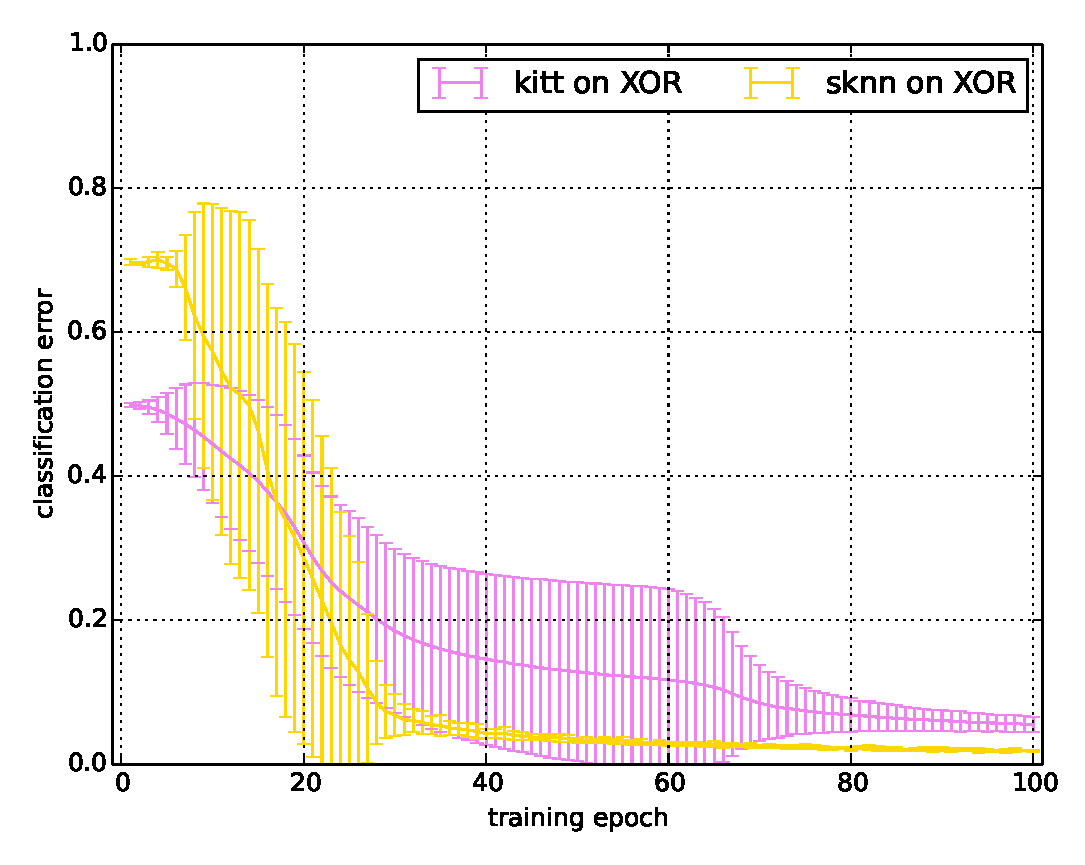
\includegraphics[width=0.8\linewidth]{kitt_verify_err}
%  \caption{Comparison of error through learning epochs to another framework (sknn).}
%  \label{fig:kitt_verify_err}
%\end{figure}

In \cref{tab:kitt_verify_f1}, the \textit{f1-score} measure (see \cref{eq:f1_score} in \cref{ssec:evaluation_methods}) is shown for individual classes (digits) of the MNIST dataset. This evaluation is done on the testing data.

\begin{table}[H]
\centering
\caption{Comparison of f1-score on MNIST to another framework (sknn)}
\label{tab:kitt_verify_f1}
\resizebox{\textwidth}{!} {
\begin{tabular}{|c|c|c|c|c|c|c|c|c|c|c|c|}
\hline
\textit{net}  & \textit{0} & \textit{1} & \textit{2} & \textit{3} & \textit{4} & \textit{5} & \textit{6} & \textit{7} & \textit{8} & \textit{9} & \textit{avg}  \\ \hline
\textbf{kitt} & 0.94       & 0.98       & 0.91       & 0.90       & 0.93       & 0.89       & 0.93       & 0.93       & 0.90       & 0.91       & \textbf{0.92} \\ \hline
\textbf{sknn} & 0.96       & 0.97       & 0.92       & 0.91       & 0.93       & 0.89       & 0.94       & 0.93       & 0.90       & 0.91       & \textbf{0.93} \\ \hline
\end{tabular}
}
\end{table}

In \cref{fig:kitt_verify_time}, a comparison of average epoch processing time is shown. The \textit{sknn} library provides an option to use \textit{gpu} in order to decrease the training time, hence also this training variant is included to the comparison.

This evaluation is done on the MNIST dataset only, as the training is quite fast on XOR for both implementations due to the smaller amount and size of samples. The average is computed out of $ 1000 $ samples, as we train $ 100 $ epochs in $ 10 $ observations.

\begin{figure}[H]
  \centering
  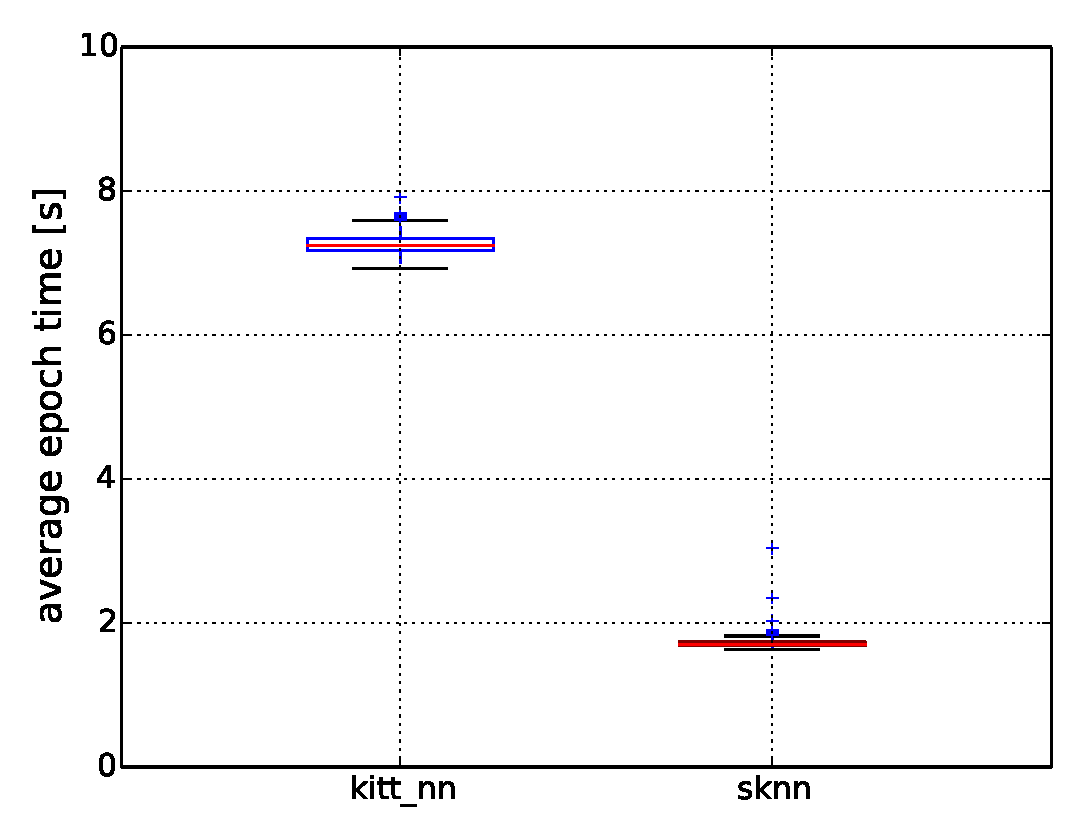
\includegraphics[width=0.8\linewidth]{kitt_verify_time}
  \caption{Comparison of average epoch processing time (1000 samples) to another framework (Scikit-neuralnetwork (sknn): \citep{misc:sknn}), MNIST dataset}
  \label{fig:kitt_verify_time}
\end{figure}

The implemented \textit{kitt\_nn} framework cannot compete in speed with the optimized stochastic \textit{GDA} of \textit{sknn} library. However, importantly for this study, the classification abilities have been verified.

\section[Performance Evaluation of the Pruning Algorithm]{Performance Evaluation of the Pruning \\Algorithm} \label{sec:pruning_algorithm_results}
This section presents results of the implemented pruning algorithm (introduced in \cref{sec:network_pruning_algorithm}). The input of the algorithm is given by a dataset and an obviously oversized neural network with a fully-connected structure. On the output, a pruned network of a minimal structure, but keeping a required classification accuracy, is expected.

The evalutaion of the algorithm is performed on the two datasets, XOR and MNIST, described in \cref{ssec:testing_datasets}.

\subsection{Evaluation on XOR Dataset} \label{ssec:evaluation_on_xor}
The XOR dataset is essential for testing the functionality of the algorithm, as we know the minimal network structure for this problem ($ [2, 2, 1] $). Initially, a network with one hidden layer of $ 100 $ neurons is constructed as the algorithm input (\cref{img:pa_xor_start}). The desired structure is shown in \cref{img:pa_xor_final}.

During the pruning process, three key network properties are observed:
\begin{enumerate}
\item network structure;
\item number of synapses in the network;
\item classification accuracy on a chosen dataset.
\end{enumerate}

Those are shown with respect to the pruning step (see the pruning loop in \cref{img:pruning_algorithm}) all together in \cref{fig:pa_result_xor}.

\begin{figure}[H]
  \centering
  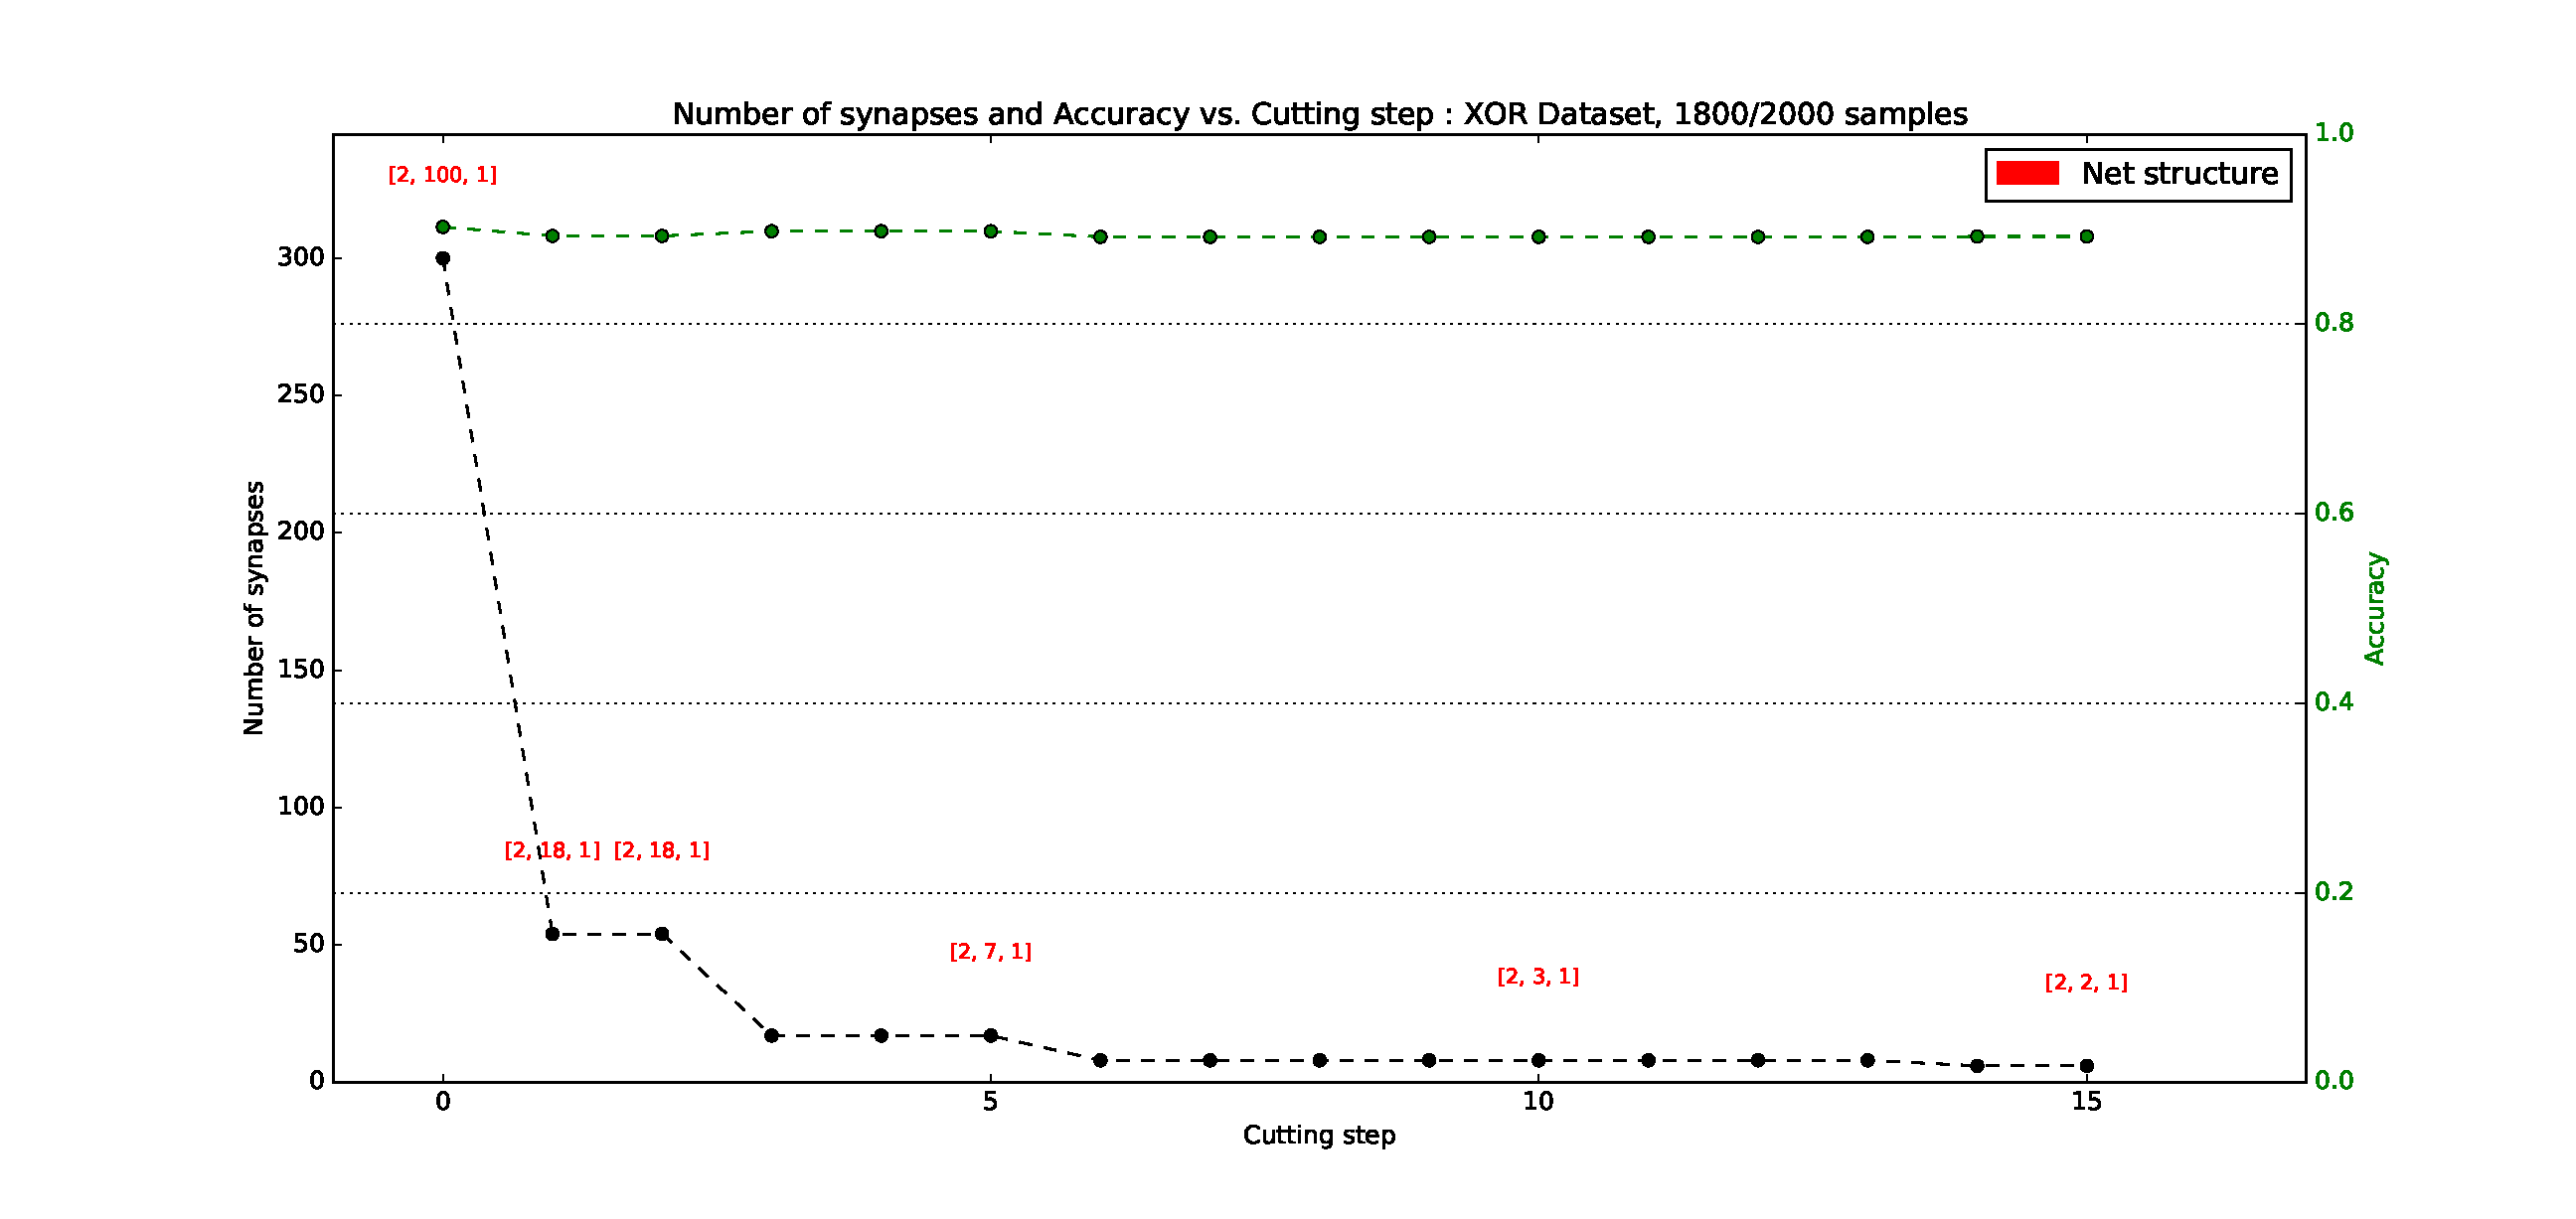
\includegraphics[width=1.0\textwidth]{pa_result_xor}
  \caption{Results of the pruning algorithm on XOR dataset.}
  \label{fig:pa_result_xor}
\end{figure}

The results are obtained by averaging $ 10 $ observations, so the outcome is independent on initial conditions. For retraining the network after a pruning step, training data is used. For verification, whether the network is capable of classification, validation data is used. Testing data is used to check the accuracy after pruning (values in \cref{fig:pa_result_xor}).

Algorithm parameters:
\begin{itemize}
\item initial network structure: $ [2, 100, 1] $;
\item required classification accuracy on validation data: $ 0.9 $;
\item learning rate: $ 0.5 $;
\item percentile levels: $ [50, 20, 5, 0] $.
\end{itemize}

Algorithm outcomes:
\begin{itemize}
\item pruning steps: $ 10 $;
\item final structure: $ [2, 2, 1] $;
\item number of removed synapses: $ 294 $ (initially: $ 300 $, finally: $ 6 $);
\item classification accuracy on testing data: $ 0.99 $.
\end{itemize}

\begin{figure}[H]
\centering
\begin{subfigure}{0.4\textwidth}
  \centering
  \includegraphics[width=0.8\linewidth]{pa_xor_start.png}
  \caption{PA input: oversized and fully-connected network}
  \label{img:pa_xor_start}
\end{subfigure}%
\begin{subfigure}{0.4\textwidth}
  \centering
  \includegraphics[width=0.8\linewidth]{pa_xor_final.png}
  \caption{PA output: minimal network structure}
  \label{img:pa_xor_final}
\end{subfigure}
\caption{PA process illustration on XOR}
\label{img:pa_xor_morph}
\end{figure}

\subsection{Evaluation on MNIST Dataset} \label{ssec:evaluation_on_mnist}
Similarly, the algorithm is evaluated on the MNIST dataset. In this case, the minimal structure is not known. The recommended size of the hidden layer for MNIST classification is $ 15 $. In \cref{fig:kitt_verify_acc} the classification accuracy of \textit{kitt\_nn} framework on this dataset is presented. Apparently, it is possible to reach a success rate around $ 90\% $. Hence these parameters are used:

\begin{itemize}
\item initial network structure: $ [784, 15, 10] $ ($ 784 $, because the samples are images of size $ 28x28 $, and $ 10 $, because we have ten digits);
\item required classification accuracy on validation data: $ 0.89 $;
\item learning rate: $ 0.1 $;
\item percentile levels: $ [50, 35, 20, 10, 5, 0] $.
\end{itemize}

\cref{fig:pa_result_mnist} shows a significant reduction of synapses while the classification accuracy is kept on $ 0.89 $. The shown results are obtained by averaging $ 10 $ observations.
\begin{figure}[H]
  \centering
  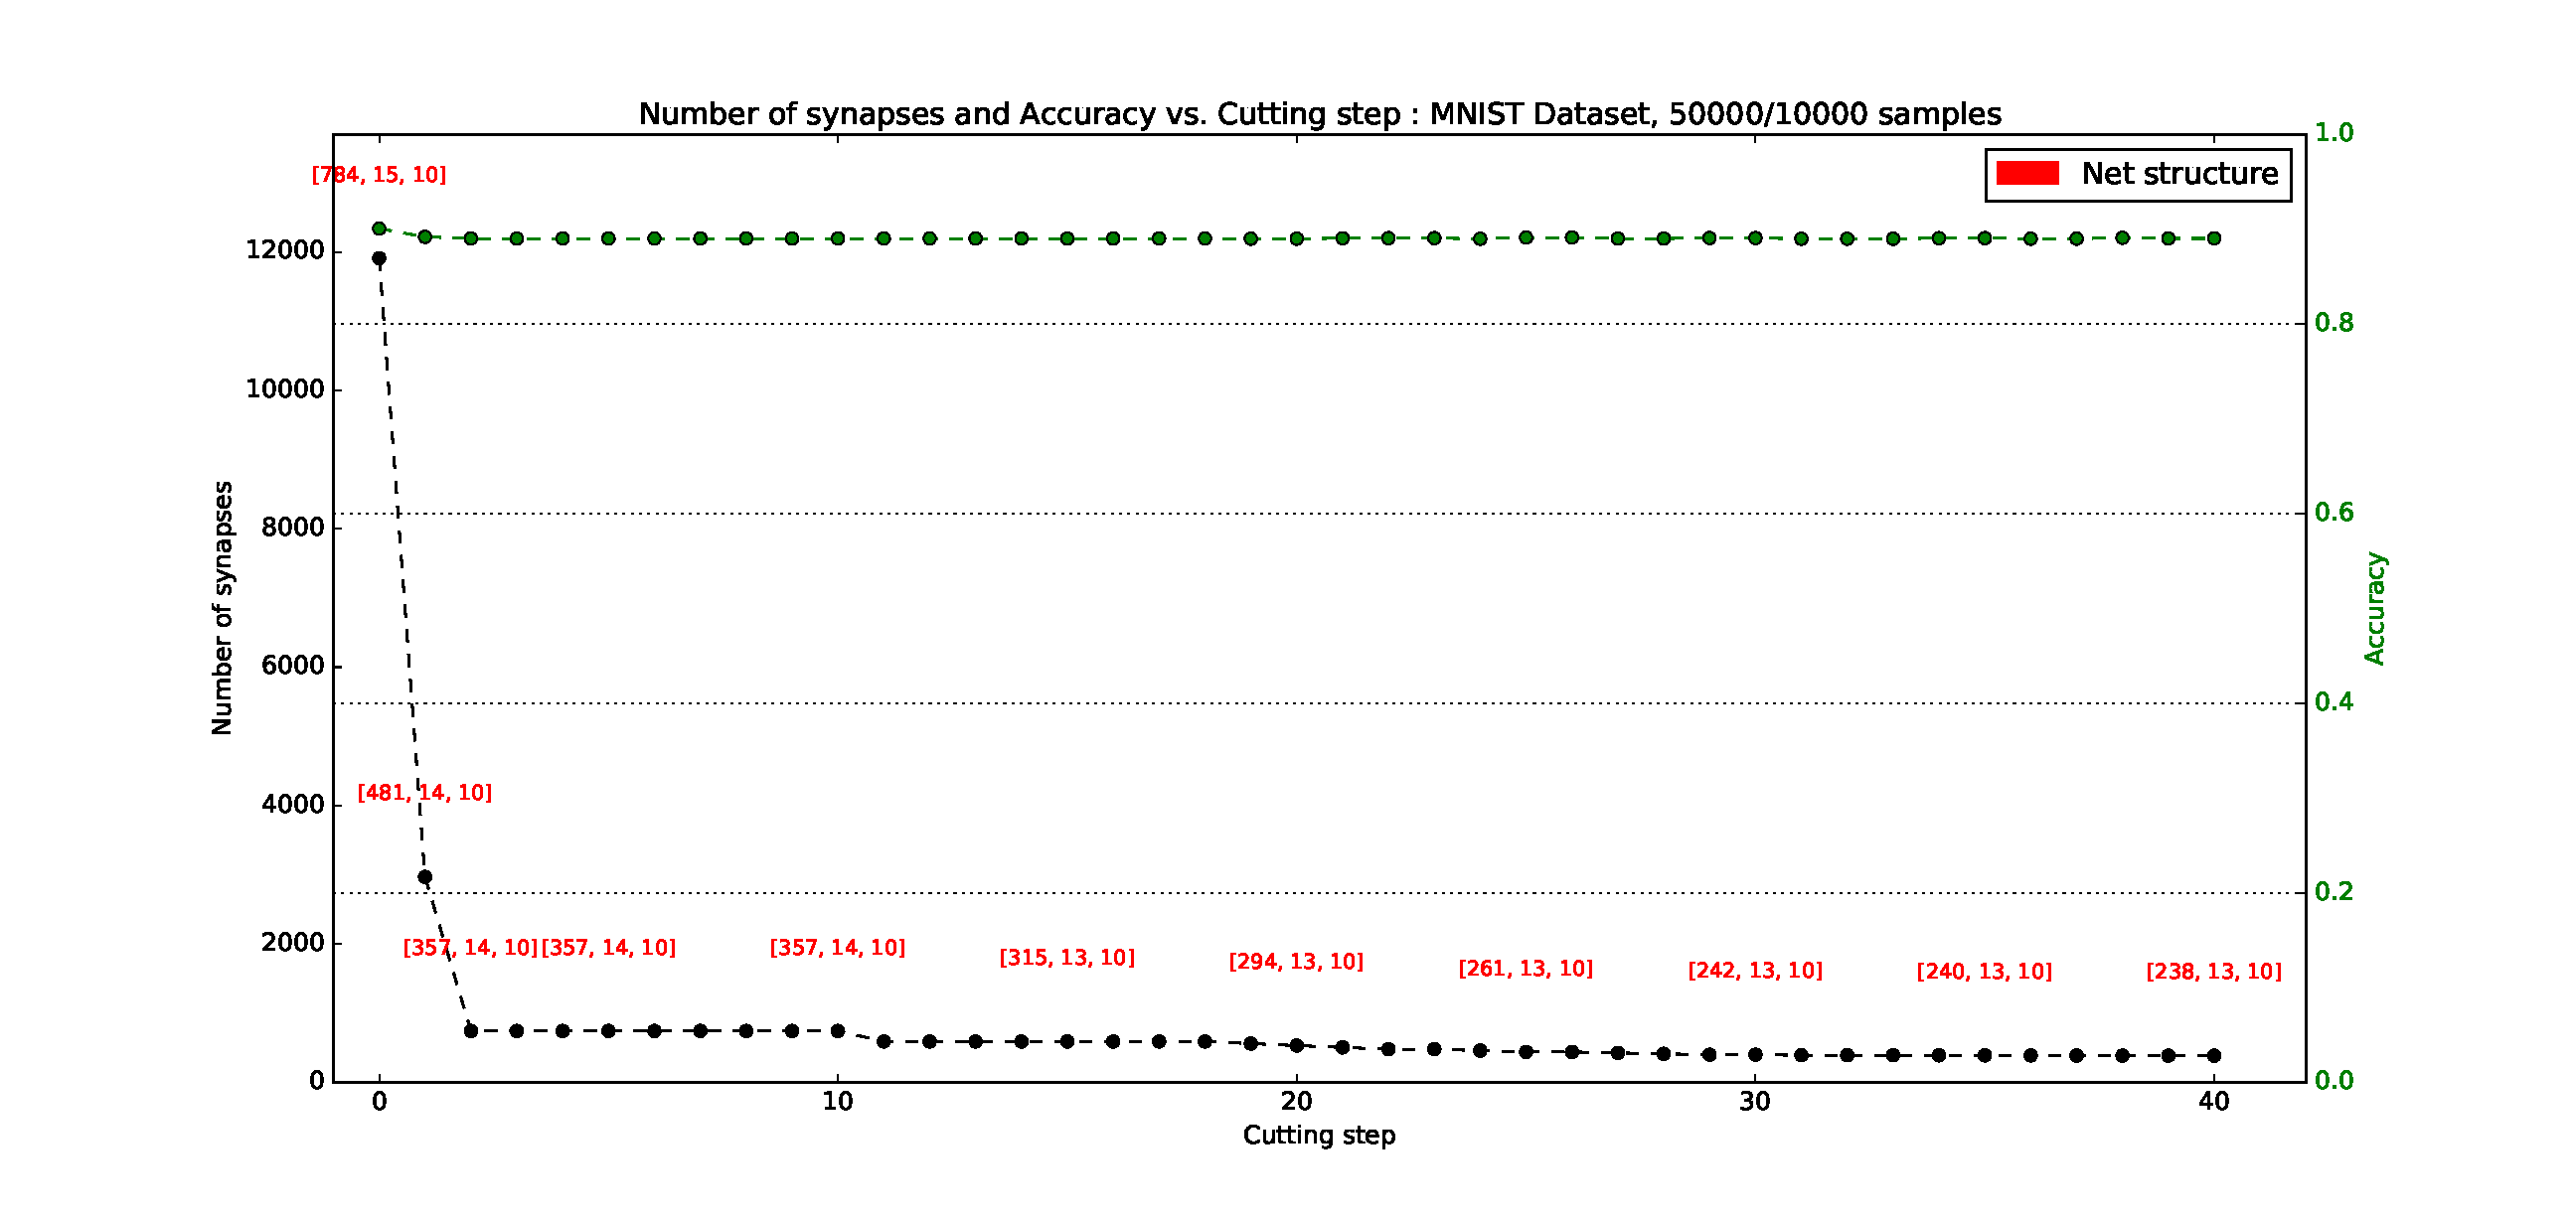
\includegraphics[width=1.0\textwidth]{pa_result_mnist}
  \caption{Pruning Algorithm Results on MNIST Dataset.}
  \label{fig:pa_result_mnist}
\end{figure}

Results of the pruning algorithm on MNIST:
\begin{itemize}
\item pruning steps: $ 76 $;
\item final structure: $ [495, 15, 10] $;
\item number of removed synapses: $ 11075 $ (initially: $ 11910 $, finally: $ 835 $, reduction: $ 92.9\% $);
\item classification accuracy on testing data: $ 0.88776 $.
\end{itemize}

The figure \ref{fig:pa_result_mnist} says that more than $ 90\% $ of the synapses in the initial network structure are redundant. Regarding the number of neurons in the network, mostly the input layer is reduced. These results make a pretty good sense, as shown in \cref{sssec:mnist_analysis}.

The following \cref{tab:pa_results_mnist} presents statistics of the first seven steps of one of the performed observations. For each step we can see the current percentile level (see \cref{img:pruning_algorithm}), corresponding reduction in the network and retraining results.

\begin{table}[H]
\centering
\caption{PA progress example on MNIST}
\label{tab:pa_results_mnist}
\resizebox{\textwidth}{!} {
\begin{tabular}{|l|c|c|c|c|c|c|c|c|}
\hline
\multicolumn{1}{|c|}{\textit{step}} & \textit{0 (initial)} & \textit{1}                  & \textit{2}                  & \textit{3}                  & \textit{4}                 & \textit{5} & \textit{6} & \textit{7} \\ \hline
percentile level                    & 50                   & 50                          & 50                          & 50                          & 50                         & 35         & 20           & 20           \\ \hline
synapses removed                    & X                    & 5955                        & 2978                        & 1489                        & 744                        & 521            & 298            & 238           \\ \hline
input neurons left                  & 784                  & 784                         & 769                         & 664                         & 464                        & 539           & 602           & 521           \\ \hline
synapses left                       & 11910                & 5955                        & 2977                        & 1488                        & 744                        & 967           & 1190           & 952           \\ \hline
acc. after pruning                  & X                    & 0.9                         & 0.887                       & 0.851                       &  0.817                      & 0.858            & 0.880           & 0.878           \\ \hline
retrained?                          & X                    & \cellcolor[HTML]{34FF34}yes & \cellcolor[HTML]{34FF34}yes & \cellcolor[HTML]{34FF34}yes & \cellcolor[HTML]{FD6864}no & \cellcolor[HTML]{FD6864}no            & \cellcolor[HTML]{34FF34}yes            & \cellcolor[HTML]{34FF34}yes            \\ \hline
epochs to retrain                   & X                    & 0                           & 4                           & 63                          & \textgreater 100           & \textgreater 100           & 8           & 12           \\ \hline
\end{tabular}
}
\end{table}

In this example, the algorithm uses the percentile level of $ 50 $ in the first three steps, meaning it cuts out the half of the synapses each time. In the fourth step, the network is not able to retrain after cutting half of the remaining synapses, hence the percentile level is decreased to $ 35 $ and less synapses are tried to be removed in the fifth step. However, the retraining is not successful again (the accuracy of $ 0.89 $ is not reached in $ 100 $ epochs), so the percentile level is decreased to $ 20 $. This time the pruned network is able to retrain, so a new structure is saved and the algorithm continues with the percentile level of $ 20 $ in the next steps.

The following figures (\ref{img:pa_mnist_morph}) illustrate the transformation of the network.
\begin{figure}[H]
\centering
\begin{subfigure}{0.4\textwidth}
  \centering
  \includegraphics[width=0.8\linewidth]{pa_mnist_start.png}
  \caption{PA input: oversized and fully-connected network}
  \label{img:pa_mnist_start}
\end{subfigure}%
\begin{subfigure}{0.4\textwidth}
  \centering
  \includegraphics[width=0.8\linewidth]{pa_mnist_final.png}
  \caption{PA output: minimal network structure}
  \label{img:pa_mnist_final}
\end{subfigure}
\caption{PA process illustration on MNIST}
\label{img:pa_mnist_morph}
\end{figure}

\subsubsection{Analysis of Minimal Structure in MNIST Dataset} \label{sssec:mnist_analysis}
As mentioned in \cref{ssec:minimal_structure_util}, minimal structures obtained from the pruning algorithm can be further researched.

For instance, considering the MNIST dataset, there is an image (meaning a vector of pixels) as the network input. As the output, there are $ 10 $ classes corresponding to digits. Having the minimal structure, one can find out which pixels are related to e.g. digit $ 7 $ class or which pixels are totally useless for classification.

As illustrated in \cref{img:structure_util}, paths from the input to the output layer can be tracked. This way we can find paths for every output neuron and see which input neurons are connected to it. Individual subpanels (a-j) in \cref{fig:mnist_analysis} show in red all input neurons (pixels of the $ 28x28 $ input images) that are connected to the corresponding output neuron (digit 0-9). Pixels having no path to the corresponding output neuron are in blue.

Subpanel (k) in \cref{fig:mnist_analysis} shows in red all pixels that have at least one path to the output layer. The blue pixels have no connection and hence do not contribute to classification.

As there are $ 15 $ hidden neurons, each input neuron can have maximally $ 15 $ connections and, naturally, minimally $ 0 $ connections in the final structure. The subpanel (l) in \cref{fig:mnist_analysis} presents the number of connections to the hidden layer for each input neuron. The results indicate that one neuron has $ 3 $ connections to the hidden layer at most. 

\begin{figure}[H]
  \centering
  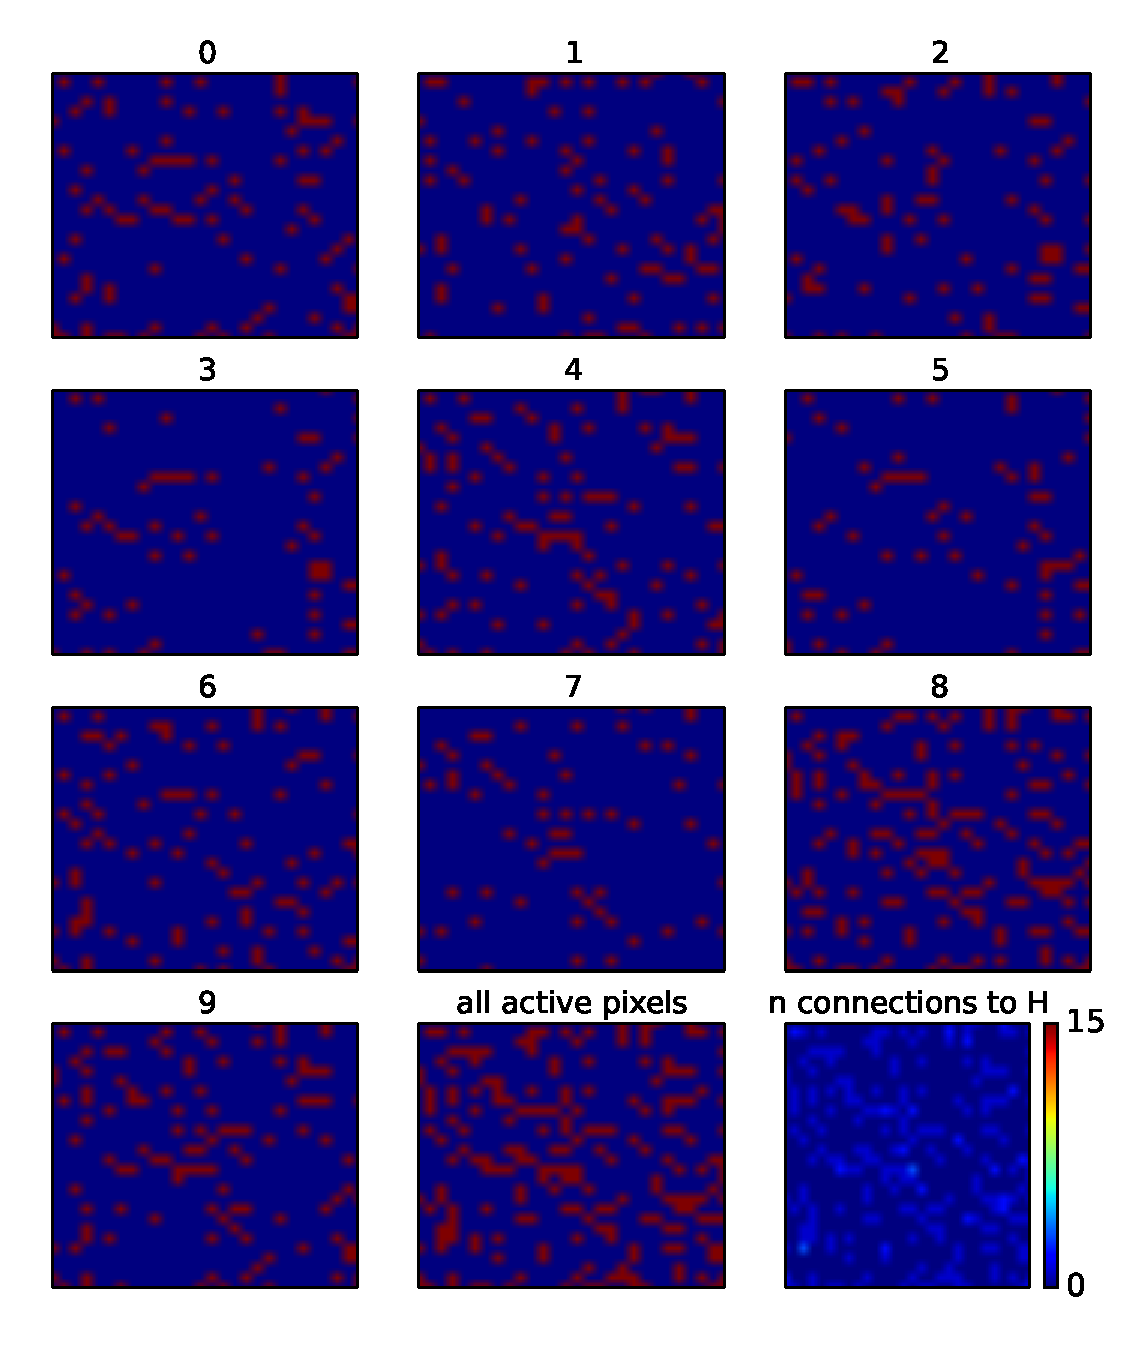
\includegraphics[width=0.6\textwidth]{fs_mnist_analysis}
  \caption{Feature Selection : MNIST Analysis.}
  \label{fig:mnist_analysis}
\end{figure}

\subsection{Comparison to Other Pruning Methods} \label{comparison_to_other_pa}
In \cref{sec:soa_pruning_algorithms}, a few approaches of network pruning are discussed. In this section, the developed pruning algorithm (PA) based on weight changes during network training (see \cref{sec:network_pruning_algorithm}) is compared to two different methods:

\begin{enumerate}[label=\Alph*]
\item \textit{pruning based on actual weight values}: The learning algorithm uses the \textit{tanh} transfer function (see \cref{fig:transfer_functions}). The pruning approach from \cref{sec:network_pruning_algorithm} is used, however, the removed synapses are chosen based on actual weight values. Synapses with weight closest to zero are removed;
\item \textit{brute force pruning algorithm}: 
In every pruning step, one synapse is removed and the network is retrained. If the retraining was unsuccessful, the synapse is put back to the network;
\end{enumerate}

\begin{figure}[H]
\centering
\begin{subfigure}{0.49\textwidth}
  \centering
  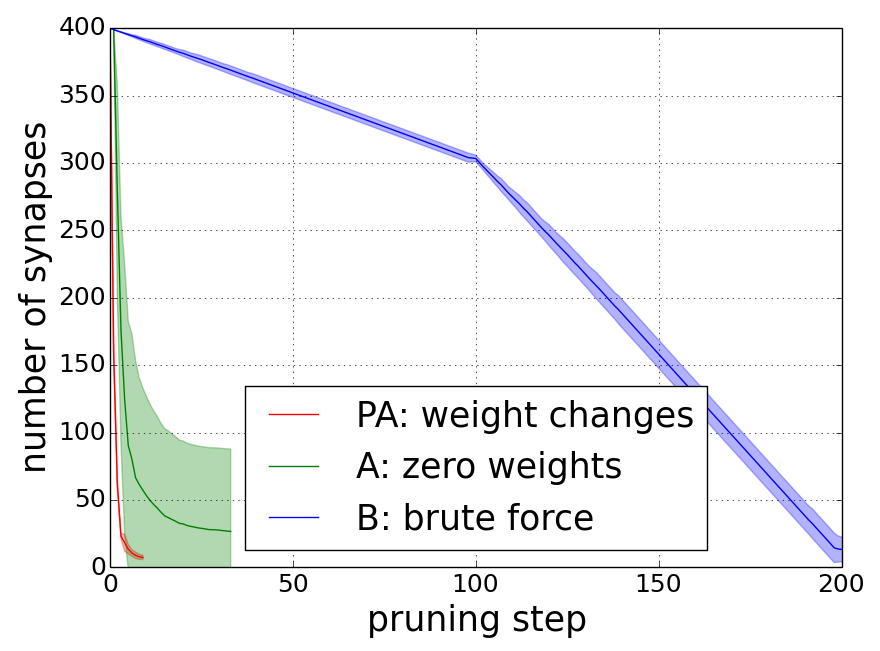
\includegraphics[width=1.0\linewidth]{pa_comparison_to_others_xor.png}
  \caption{comparison on XOR}
  \label{fig:pa_comparison_xor}
\end{subfigure}%
\begin{subfigure}{0.49\textwidth}
  \centering
  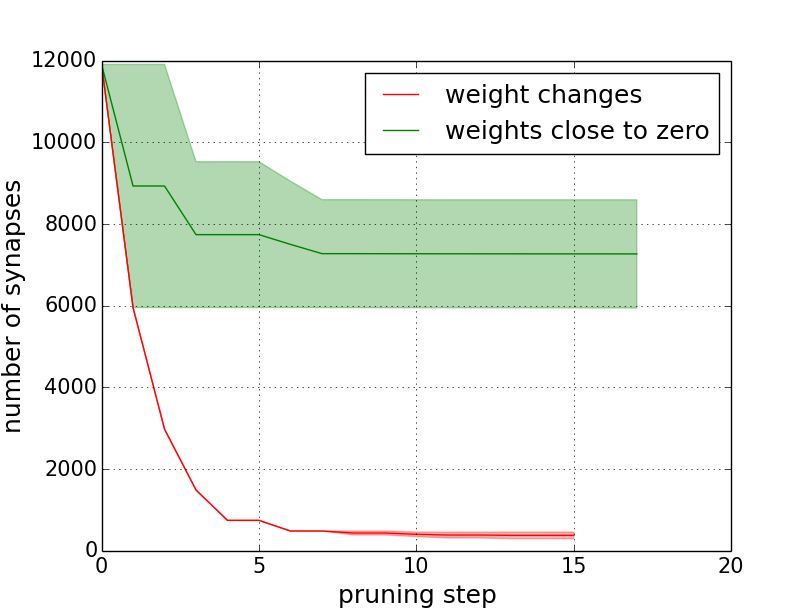
\includegraphics[width=1.0\linewidth]{pa_comparison_to_others_mnist.png}
  \caption{comparison on MNIST}
  \label{fig:pa_comparison_mnist}
\end{subfigure}
\caption{Comparison of the developed PA to other pruning methods (10 observations).}
\label{fig:pa_comparison}
\end{figure}

The comparison was performed on XOR and on MNIST (see \cref{ssec:testing_datasets}) by averaging results of 10 observations. The brute force approach (B) was only done on XOR as it would take up to 11910 pruning steps and a long evaluation time on MNIST. Regarding its performance on XOR, only one synapse is removed in each of the first $ 98 $ steps. Then, removing also the second synapse coming to a hidden neuron, this neuron dies as it has no input, hence also synapses on its output are removed. Therefore more synapses are removed per step after $ 98^{th} $ iteration as shown in \cref{fig:pa_comparison_xor}. The minimal structure is always found by the brute force approach.

Regarding the approach (A), finding the minimal structure is not guaranteed (see \cref{tab:pa_comparison}). Apparently, the way of selecting removed synapses is not correct, which indicates that even synapses with a low weight may be important. 

\begin{table}[H]
\centering
\caption{Comparison of the developed PA to other pruning methods (10 observations). Required accuracy on validation data: XOR: 0.99, MNIST: 0.85.}
\label{tab:pa_comparison}
\resizebox{\textwidth}{!} {
\begin{tabular}{|l|c|c|c|c|c|c|c|c|}
\hline
\multirow{2}{*}{} & \multicolumn{4}{c|}{\textit{XOR}}                                           & \multicolumn{4}{c|}{\textit{MNIST}}                      \\ \cline{2-9} 
                  & \textit{steps} & \textit{synapses} & \textit{structure} & \textit{accuracy} & \textit{steps} & synapses & structure         & accuracy \\ \hline
PA                & 10             & 6                 & {[}2, 2, 1{]}      & 0.9795            & 16             & 377      & {[}252, 15, 10{]} & 0.8396   \\ \hline
A                 & 34             & 27                & {[}2, 8, 1{]}      & 0.9875            & 18             & 7269     & {[}784, 15, 10{]} & 0.6471   \\ \hline
B                 & 218            & 6                 & {[}2, 2, 1{]}      & 0.9685            & \multicolumn{4}{c|}{X}                                   \\ \hline
\end{tabular}}
\end{table}

\section{Results of Terrain Classification} \label{sec:terrain_processing_results}
In this section, results of the overall terrain classification process (see \cref{chap:terrain_classification}) are presented and the global process parameters are analysed.  

First of all, complete classification results based on the generated datasets are listed and more detailed results of a deterministic configuration (with no noise) are  compared to a realistic noisy configuration. Different classification methods are also applied on the noisy dataset for comparison.

In \cref{ssec:selection_of_learning_parameters}, the way of finding optimal learning parameters is presented. Then, an analysis of terrain noise and signal noise influence is done in \cref{ssec:influence_of_noise_on_classification} and time needed for classification is determined in \cref{ssec:number_of_timesteps}. Classification using separately different sensor types is evaluated in \cref{ssec:analysis_of_used_sensor_types}. Finally, terrain classification results based on proprioceptive and tactile sensing are compared to vision-based methods in \cref{ssec:terrain_classification_vs_soa}.

\subsection{Classification Performance} \label{ssec:classification_performance}
The generated datasets, differing one from each other in the global process parameters, are listed in \cref{app:tab:generated_datasets}. For each of them, $ 10 $ observations of the classification process were performed and the classification results presented in \cref{tab:classification_results} were computed by averaging these observations.

Based on the analysis in \cref{ssec:selection_of_learning_parameters}, the network hidden structure consisted of $ 1 $ layer with $ 20 $ neurons. The backpropagation learning rate was $ 0.5 $ and the training process lasted for $ 500 $ learning epochs.

With reference to \cref{app:tab:generated_datasets}, dataset $ 00\_00\_40\_a $ (meaning no terrain noise, no signal noise, 40 timesteps and all sensors) was selected for more detailed analysis. Classification results on this dataset are considered as a reference, because the data is deterministic and the results best possible.

\begin{table}[H]
\centering
\caption{Classification results on generated datasets (see dataset parameters in \cref{app:tab:generated_datasets}).}
\label{tab:classification_results}
\resizebox{\textwidth}{!} {
\begin{tabular}{|c|c|c|c|c|c|c|}
\hline
\textit{dataset} & \textit{accuracy} & \textit{precision} & \textit{recall} & \textit{f1-score} & \textit{error} & \textit{ep. time {[}s{]}} \\
\hline
00\_00\_80\_p 	& 0.624 	& 0.596 	& 0.624 	& 0.576 	& 0.072 	& 1.089 	 \\ \hline
00\_00\_80\_a 	& 0.922 	& 0.920 	& 0.920		& 0.920 	& 0.020 	& 1.330 	 \\ \hline
00\_03\_40\_a 	& 0.902 	& 0.900 	& 0.900 	& 0.900 	& 0.019 	& 0.765 	 \\ \hline
00\_00\_30\_a 	& 0.847 	& 0.840 	& 0.848 	& 0.842 	& 0.030 	& 0.964 	 \\ \hline
00\_00\_10\_p 	& 0.489 	& 0.468 	& 0.490 	& 0.430 	& 0.089 	& 0.565 	 \\ \hline
00\_01\_40\_a 	& 0.776 	& 0.790 	& 0.780 	& 0.760 	& 0.040 	& 0.751 	 \\ \hline
00\_00\_01\_a 	& 0.639 	& 0.646 	& 0.638 	& 0.624 	& 0.073 	& 0.526 	 \\ \hline
00\_00\_80\_t	& 0.761 	& 0.764 	& 0.760 	& 0.742 	& 0.051 	& 0.715 	 \\ \hline
00\_00\_20\_a 	& 0.850 	& 0.848 	& 0.850 	& 0.846 	& 0.030 	& 0.894 	 \\ \hline
00\_05\_40\_a 	& 0.884 	& 0.880 	& 0.880 	& 0.880 	& 0.019 	& 0.760 	 \\ \hline
00\_00\_40\_a 	& 0.923 	& 0.920 	& 0.920 	& 0.920 	& 0.019 	& 0.865 	 \\ \hline
00\_00\_10\_a 	& 0.805 	& 0.806 	& 0.804 	& 0.798 	& 0.040 	& 0.526 	 \\ \hline
00\_00\_40\_p 	& 0.696 	& 0.702 	& 0.694 	& 0.666 	& 0.060 	& 0.707 	 \\ \hline
00\_00\_10\_t 	& 0.423 	& 0.432 	& 0.424 	& 0.386 	& 0.102 	& 0.469 	 \\ \hline
00\_10\_40\_a 	& 0.851 	& 0.850 	& 0.850 	& 0.850 	& 0.026 	& 0.792 	 \\ \hline
00\_00\_40\_t	& 0.701 	& 0.692 	& 0.702 	& 0.670 	& 0.064 	& 0.475 	 \\ \hline
01\_03\_40\_a 	& 0.772 	& 0.780 	& 0.770 	& 0.760 	& 0.044 	& 1.314 	 \\ \hline
01\_10\_40\_a 	& 0.639 	& 0.670 	& 0.640 	& 0.630 	& 0.060 	& 0.944 	 \\ \hline
01\_01\_40\_a 	& 0.759 	& 0.770 	& 0.760 	& 0.750 	& 0.052 	& 1.093 	 \\ \hline
01\_00\_40\_a 	& 0.815 	& 0.830 	& 0.810 	& 0.820 	& 0.041 	& 0.844 	 \\ \hline
01\_05\_40\_a 	& 0.780 	& 0.790 	& 0.780 	& 0.770 	& 0.044 	& 0.900 	 \\ \hline
03\_10\_40\_a 	& 0.565 	& 0.530 	& 0.560 	& 0.540 	& 0.063 	& 0.946 	 \\ \hline
03\_05\_40\_a 	& 0.645 	& 0.640 	& 0.650 	& 0.630 	& 0.054 	& 0.871 	 \\ \hline
03\_00\_40\_a 	& 0.714 	& 0.730 	& 0.710 	& 0.700 	& 0.057 	& 0.831 	 \\ \hline
03\_03\_40\_a 	& 0.719 	& 0.740 	& 0.720 	& 0.720 	& 0.046 	& 0.939 	 \\ \hline
03\_01\_40\_a 	& 0.779 	& 0.780 	& 0.780 	& 0.780 	& 0.042 	& 1.068 	 \\ \hline
05\_01\_40\_a	& 0.732 	& 0.740 	& 0.730 	& 0.730 	& 0.052 	& 1.018 	 \\ \hline
05\_05\_40\_a 	& 0.651 	& 0.660 	& 0.650 	& 0.640 	& 0.056 	& 0.933 	 \\ \hline
05\_10\_40\_a 	& 0.601 	& 0.610 	& 0.600 	& 0.600		& 0.062 	& 0.954 	 \\ \hline
05\_03\_40\_a 	& 0.677 	& 0.710 	& 0.680 	& 0.670 	& 0.052 	& 0.949 	 \\ \hline
05\_00\_40\_a 	& 0.685 	& 0.720 	& 0.690 	& 0.680 	& 0.055 	& 0.835 	 \\ \hline
10\_10\_40\_a 	& 0.459 	& 0.460 	& 0.460 	& 0.430 	& 0.087 	& 0.983 	 \\ \hline
10\_03\_40\_a	& 0.621 	& 0.630 	& 0.620 	& 0.600 	& 0.070 	& 0.824 	 \\ \hline
10\_01\_40\_a 	& 0.594 	& 0.630 	& 0.590 	& 0.580 	& 0.072 	& 1.131 	 \\ \hline
10\_00\_40\_a 	& 0.614 	& 0.610 	& 0.610 	& 0.590 	& 0.067 	& 0.822 	 \\ \hline
10\_05\_40\_a 	& 0.543 	& 0.580 	& 0.540 	& 0.530 	& 0.074 	& 0.875 	 \\ \hline
20\_01\_40\_a 	& 0.459 	& 0.480 	& 0.460 	& 0.440 	& 0.093 	& 1.071 	 \\ \hline
20\_00\_40\_a 	& 0.463 	& 0.470 	& 0.460 	& 0.440 	& 0.087 	& 0.827 	 \\ \hline
20\_05\_40\_a 	& 0.436 	& 0.450 	& 0.440 	& 0.410 	& 0.091 	& 0.947 	 \\ \hline
20\_10\_40\_a 	& 0.371 	& 0.360 	& 0.370 	& 0.360 	& 0.090 	& 0.993 	 \\ \hline
20\_03\_40\_a	& 0.439 	& 0.470 	& 0.440 	& 0.420 	& 0.091 	& 0.923 	 \\ \hline
\end{tabular}
}
\end{table}

The following \cref{fig:amter_cm_nn} illustrates a confusion matrix (see \cref{ssec:evaluation_measures}) for classification on the reference deterministic dataset ($ 00\_00\_40\_a $). The recall rate for all terrains is shown on the diagonal. Additionally, we can see that $ 15\% $ of carpet samples was mistakenly labeled as grass and $ 10\% $ of grass samples as carpet. Similarly, the network had difficulties to distuinguish rock from grass and wood or foam from swamp. However, in general, the classification on the deterministic dataset was successful.

\begin{figure}[H]
  \centering
  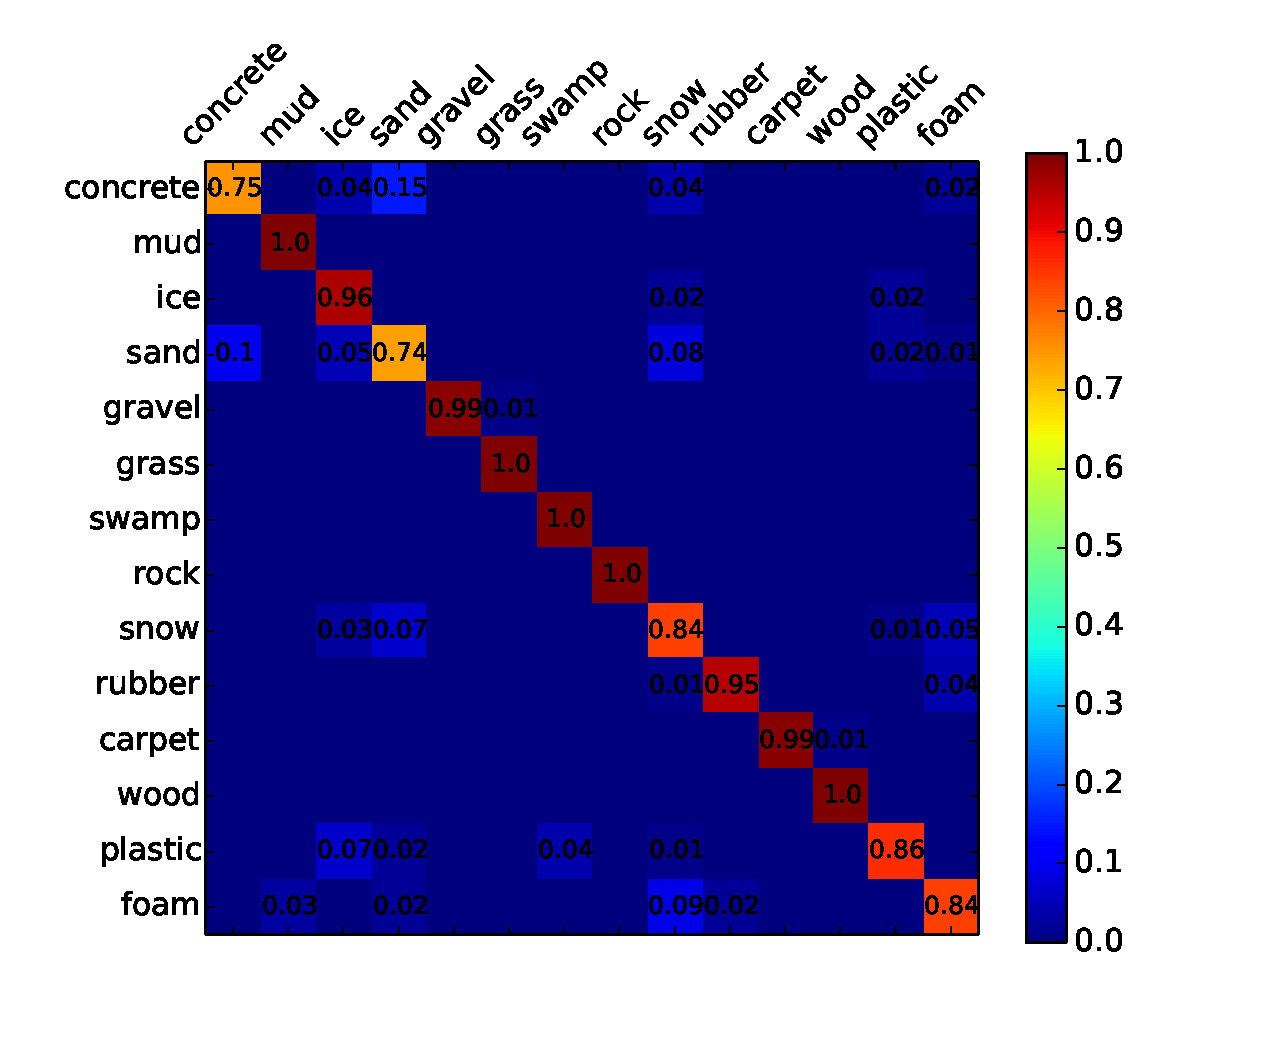
\includegraphics[width=0.7\textwidth]{amter_classification_nn_cm}
  \caption{Confusion matrix of classification results on a deterministic dataset.}
  \label{fig:amter_cm_nn}
\end{figure}

\cref{fig:amter_cm_noisy} shows a confusion matrix of classification results on a noisy dataset $ 03\_03\_40\_a $ ($ 3\% $ relative terrain noise, $ 3\% $ relative signal noise, 40 timesteps and all sensors - see \cref{app:tab:generated_datasets}).

\begin{figure}[H]
  \centering
  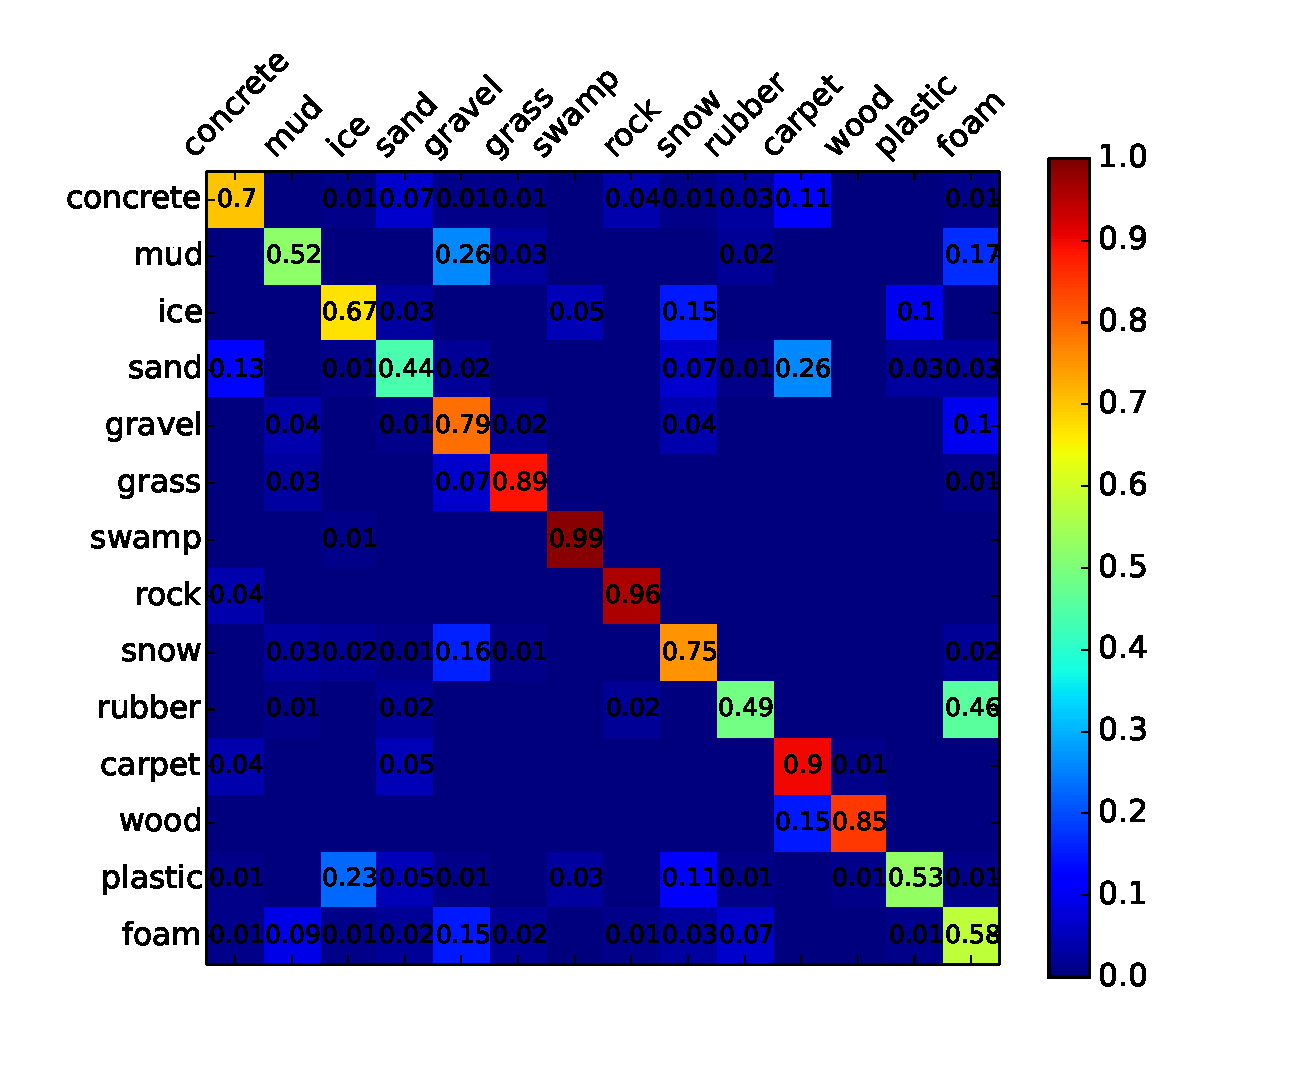
\includegraphics[width=0.7\textwidth]{amter_classification_noisy_cm}
  \caption{Confusion matrix of classification results on a noisy dataset.}
  \label{fig:amter_cm_noisy}
\end{figure}

A complete analysis of the relation between noise level and classification performance is presented in \cref{ssec:influence_of_noise_on_classification}. However, assuming that the chosen noise level simulates a real environment, \cref{fig:amter_cm_noisy} predicts results of the method on the real platform.

In this case, grass ($ 44\% $) and rubber ($ 49\% $) result with the worst recall. On the other hand, samples of mud, plastic or sand are classified very well. A complete classification report comparing the deterministic results to noisy results is shown in \cref{tab:amter_classification_report}.

\begin{table}[H]
\centering
\caption{Classification report for a deterministic dataset and a noisy dataset.}
\label{tab:amter_classification_report}
\begin{tabular}{|l|c|c|c|c|c|} 
\hline
\multirow{2}{*}{} & \multicolumn{2}{c |}{deterministic data} & \multicolumn{2}{c |}{noisy data} & \multirow{2}{*}{\textit{support}} \\ \cline{2-5} 
& \textit{precision} & \textit{recall} & \textit{precision} & \textit{recall} & \\
\hline
     carpet &      0.88 &      0.75 &     0.75 &       0.70 &       100 \\ \hline
   concrete &      0.97 &      1.00 &     0.72 &       0.52 &       100 \\ \hline
       foam &      0.83 &      0.96 &     0.70 &       0.67 &       100 \\ \hline
      grass &      0.74 &      0.74 &     0.63 &       0.44 &       100 \\ \hline
     gravel &      1.00 &      0.99 &     0.54 &       0.79 &       100 \\ \hline
        ice &      0.99 &      1.00 &     0.91 &       0.89 &       100 \\ \hline
        mud &      0.96 &      1.00 &     0.93 &       0.99 &       100 \\ \hline
    plastic &      1.00 &      1.00 &     0.93 &       0.96 &       100 \\ \hline
       rock &      0.77 &      0.84 &     0.65 &       0.75 &       100 \\ \hline
     rubber &      0.98 &      0.95 &     0.78 &       0.49 &       100 \\ \hline
       sand &      1.00 &      0.99 &     0.63 &       0.90 &       100 \\ \hline
       snow &      0.99 &      1.00 &     0.98 &       0.85 &       100 \\ \hline
      swamp &      0.95 &      0.86 &     0.79 &       0.53 &       100 \\ \hline
       wood &      0.88 &      0.84 &     0.42 &       0.58 &       100 \\ \hline
\hline \hline
avg / total &      0.92 &      0.92 &     0.74  &      0.72 & 		1400\\
\hline
\end{tabular}
\end{table}

\subsubsection{Comparison to Other Classification Methods}
Using the noisy dataset $ 03\_03\_40\_a $, the classification performance of the developed framework \textit{KITTNN} was compared to other classification approaches presented in \cref{sec:soa_other_classifiers} (\cref{tab:tc_comparison_to_other_classification_methods}).

\begin{table}[H]
\centering
\caption{Comparison to other classification methods (presented in \cref{sec:soa_other_classifiers})}
\label{tab:tc_comparison_to_other_classification_methods}
\begin{tabular}{|l|l|c|c|c|c|} 
\hline
method & method param & \textit{accuracy} & \textit{precision} & \textit{recall} & \textit{f1-score} \\
\hline \hline
   KITTNN 	&  hidden neurons: 20 	 &     0.719 &      0.740 &      0.720 &   0.720\\ \hline
   SKNN     &  hidden neurons: 20 	 &     0.812 &      0.820 &      0.810 &   0.810\\ \hline
   RF       &  estimators: 10		 &     0.647 &      0.650 &      0.650 &   0.640\\ \hline
   SVM      &  penalty: 1.0			 &     0.545 &      0.570 &      0.550 &   0.500\\ \hline
   k-NN     &  neighbours: 10	 	 &     0.733 &      0.740 &      0.730 &   0.720\\ \hline
\hline
\end{tabular}
\end{table}

The comparison to \textit{SKNN} indicates that the \textit{KITTNN} implementation might be optimizable. However, in general, the results prooved the suitability of using neural networks.

\subsection{Selection of Learning Parameters} \label{ssec:selection_of_learning_parameters}
This section is devoted to an analysis of parameters belonging to the network and the learning process. The goal was to determine:

\begin{enumerate}
\item hidden structure of the network;
\item learning rate for the backpropagation;
\item number of learning epochs (iterations).
\end{enumerate}

To perform the analysis, the deterministic dataset ($ 00\_00\_40\_a $ - see \cref{app:tab:generated_datasets}) was used.

\begin{figure}[H]
  \centering
  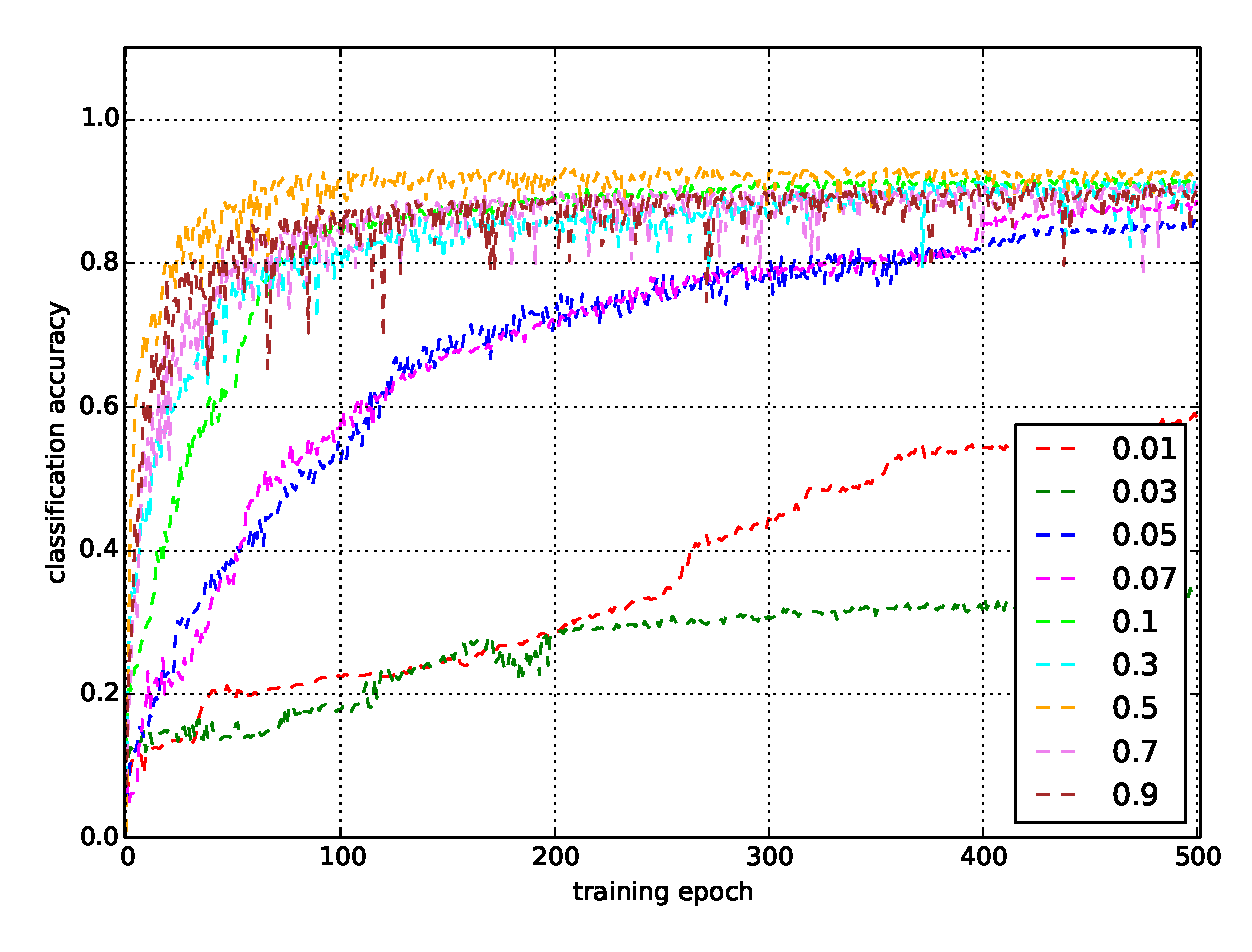
\includegraphics[width=0.7\textwidth]{cl_lr_vs_epoch_st20}
  \caption{Training process with various learning rates.}
  \label{fig:lr_analysis}
\end{figure}

In \cref{fig:lr_analysis}, the training process (progress of accuracy over iterations) is illustrated for five learning rates. The results are obtained by averaging $ 10 $ observations and (standard deviation) error bars are shown. The experiment was performed using a network with $ 20 $ hidden neurons.

\begin{figure}[H]
  \centering
  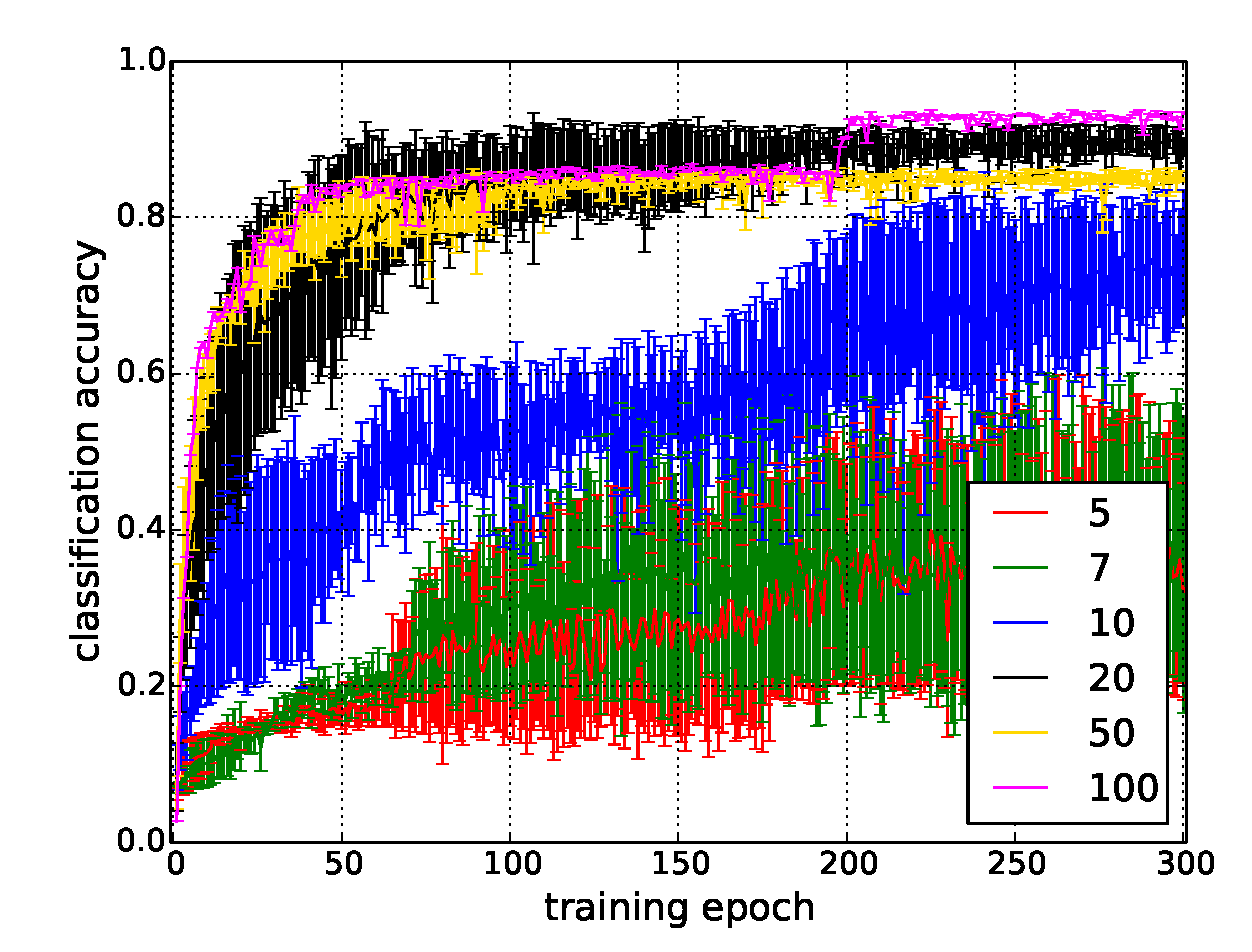
\includegraphics[width=0.7\textwidth]{cl_st_vs_epoch_lr05}
  \caption{Training process with various networks differing in the number of hidden neurons.}
  \label{fig:st_analysis}
\end{figure}

It was determined to use one hidden layer. The accuracy progress over training epochs for six networks differing in the number of hidden neurons is shown in \cref{fig:st_analysis}. An overall analysis for these two parameters (learning rate and hidden structure) is performed in \cref{fig:acc_st_lr_mat}.

\begin{figure}[H]
  \centering
  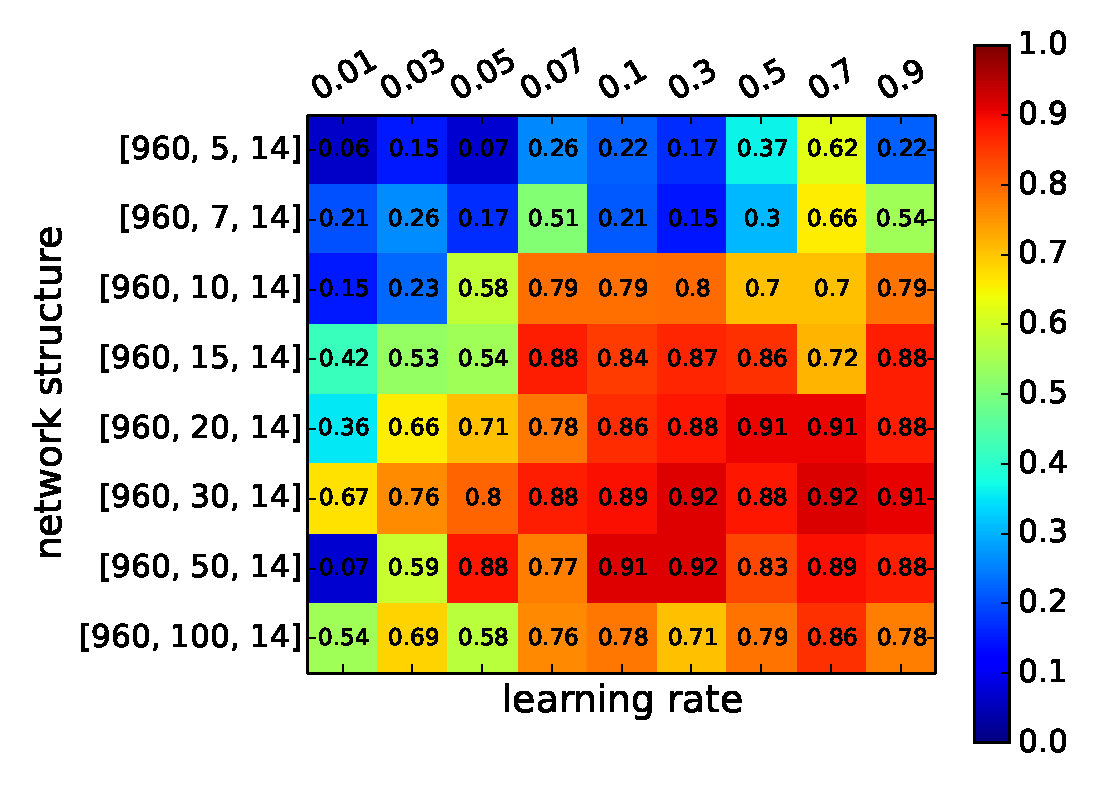
\includegraphics[width=0.8\textwidth]{cl_st_lr_mat}
  \caption{Classification accuracy vs. learning rate and network structure (10 observations)}
  \label{fig:acc_st_lr_mat}
\end{figure}

Based on the results, $ 20 $ neurons in one layer were chosen to form the hidden structure of the network. The learning rate was set to $ 0.5 $. The number of training epochs (based on \cref{fig:lr_analysis} and \cref{fig:st_analysis}) was set to $ 500 $.

\subsection{Influence of Noise on Classification} \label{ssec:influence_of_noise_on_classification}
Two types of noise were added to the deterministic data during the process: a terrain noise (described in \cref{ssec:terrain_noise}) and a signal noise (\cref{ssec:signal_noise}). Both were parametrized by a standard deviation value. \cref{fig:acc_tn_sn_mat} shows the influence of these values on classification performance.

\begin{figure}[H]
  \centering
  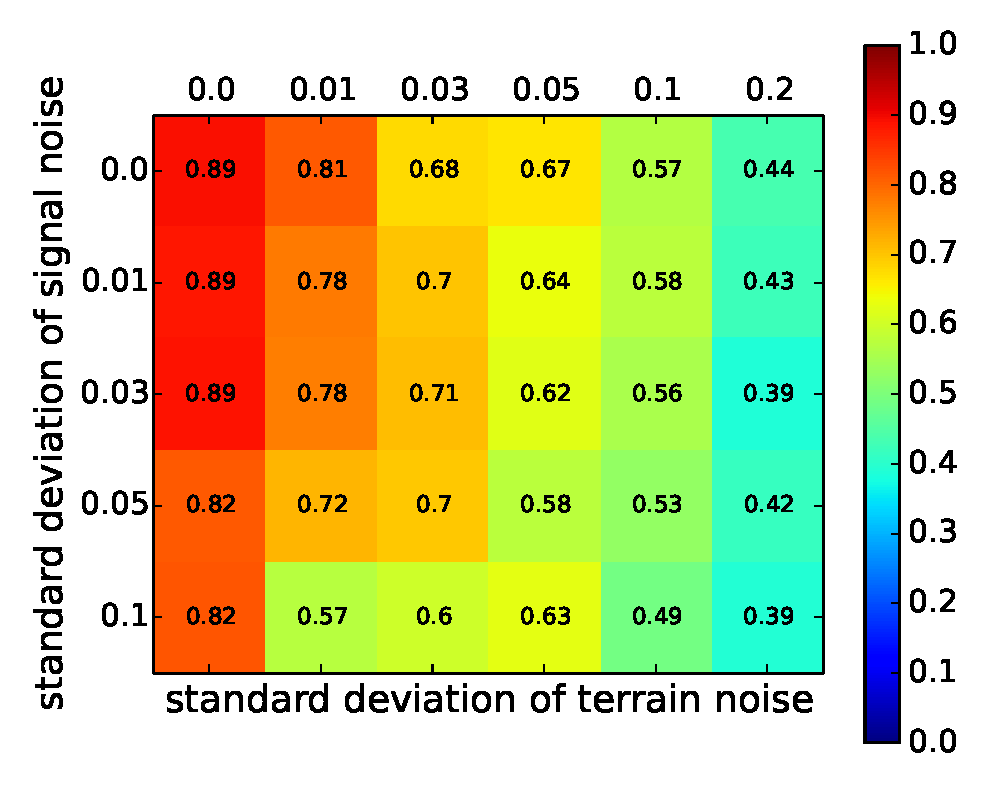
\includegraphics[width=0.7\textwidth]{cl_acc_tn_sn_mat}
  \caption{Additive terrain and signal noise: influence on the accuracy}
  \label{fig:acc_tn_sn_mat}
\end{figure}

\subsection{Time Needed for Classification} \label{ssec:number_of_timesteps}
As discussed in \cref{sec:data_acquisition}, the assumption is that the robot needs to make several steps and record the sensory data over a period of time, to classify the terrain with proprioceptive and tactile sensors. In this section, the period of time needed for proper classification is analysed. Assuming that one second in reality is equal to $ 10 $ simulation steps, \cref{fig:ts_acc_boxplot} shows the classification accuracy for six different numbers of simulation steps. The classification was performed on the deterministic dataset ($ 00\_00\_40\_a $ - see \cref{app:tab:generated_datasets}).

\begin{figure}[H]
  \centering
  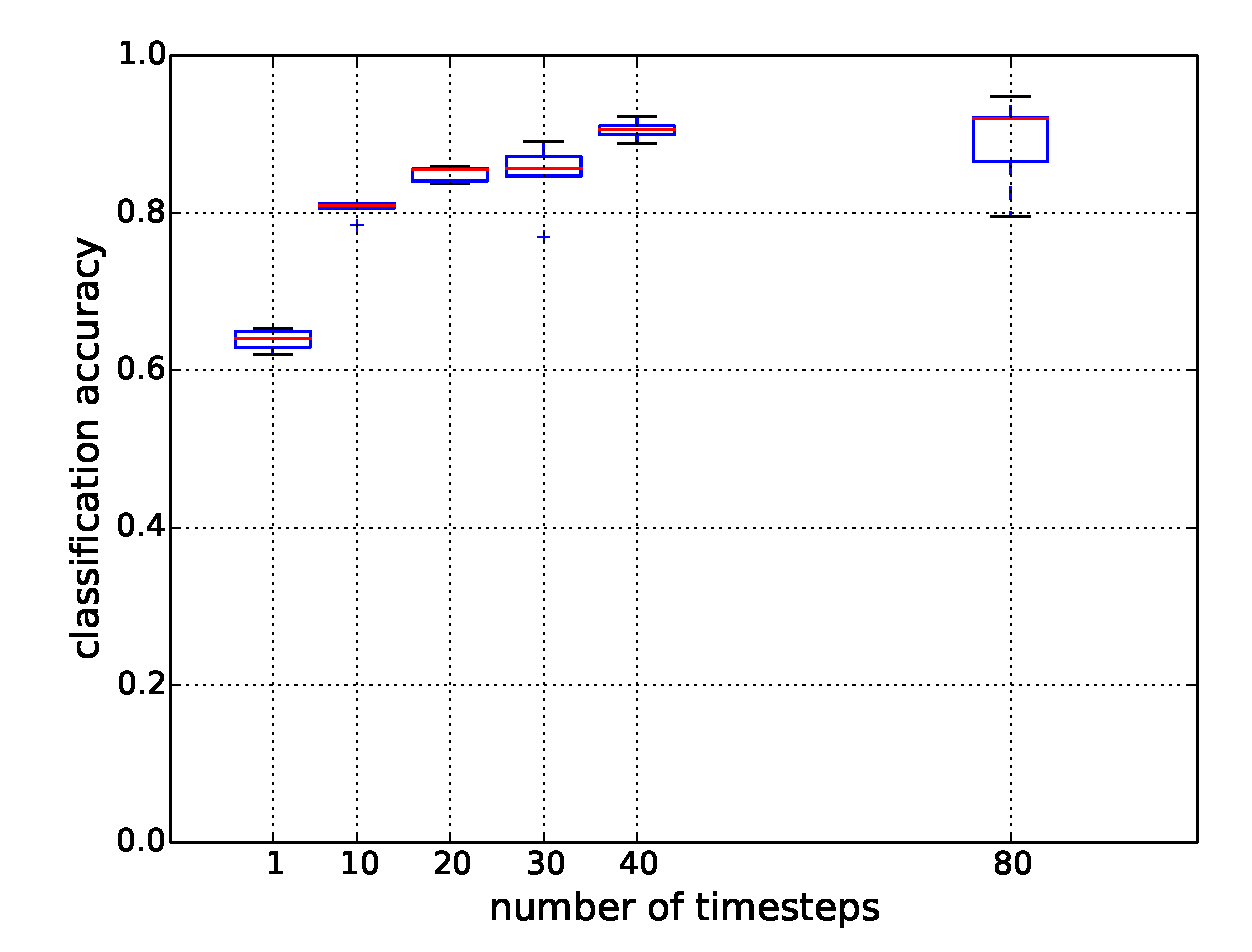
\includegraphics[width=0.75\textwidth]{cl_ts_acc_boxplot}
  \caption{Analysis of time needed for proper classification.}
  \label{fig:ts_acc_boxplot}
\end{figure}

Surprisingly, the classification result based on a single timestep is not bad. In other words, the robot will be able to classify the terrain in real time with more than $ 0.6 $ probability of success. In general, the more timesteps are used, the better the result is.

\begin{figure}[H]
  \centering
  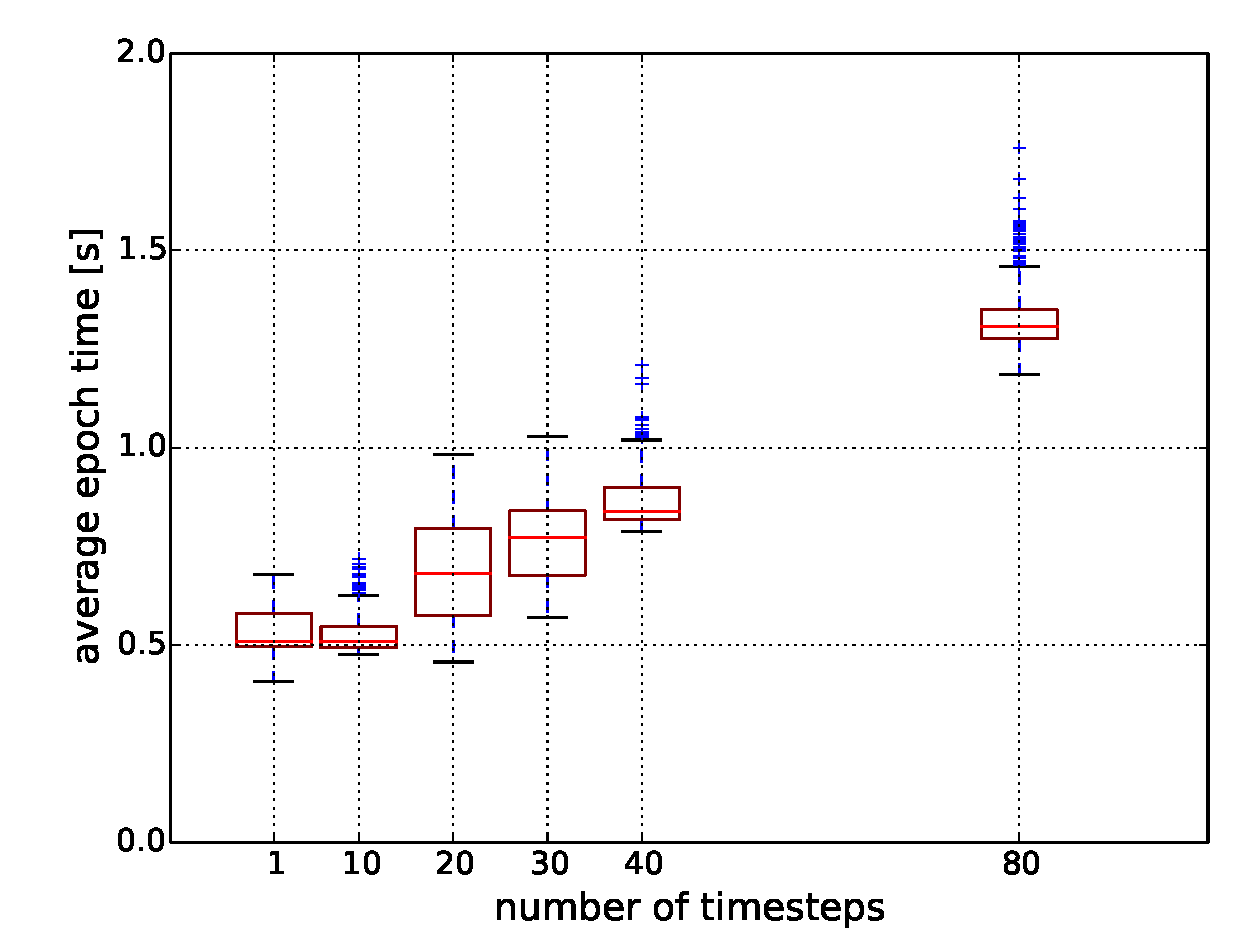
\includegraphics[width=0.7\textwidth]{cl_ts_time_boxplot}
  \caption{Average epoch time (10 observations) with respect to number of simulation timesteps.}
  \label{fig:ts_time_boxplot}
\end{figure}

However, the equally good results for $ 40 $ and $ 80 $ timesteps indicates, that one period of the tripod gait will be enough (see the periodic sensory signals in \cref{app:sec:complete_sensory_data}). Moreover, with the increasing number of timesteps, also the feature vector size and network dimensionality increase, and, as shown in \cref{fig:ts_time_boxplot}, also the processing time. Based on this analysis, $ 40 $ was chosen as the default number of timesteps in this study. 

\subsection{Analysis of Used Sensor Types} \label{ssec:analysis_of_used_sensor_types}
Two types of sensors are used for terrain classification for the hexapod robot AMOS II:

\begin{enumerate}
\item proprioceptive sensors (3 on each leg, 18 in total);
\item tactile sensors (1 on each leg, 6 in total).
\end{enumerate}

The results presented so far are obtained using both of these two types together. In this section, the sensor types are evaluated separately. \cref{fig:sen_vs_epoch} illustrates the training process using the sensor types one by one and compares their classification performance to a combined configuration. The evaluation is performed for three values of simulation timesteps (see \cref{ssec:number_of_timesteps}): $ 10 $, $ 40 $, $ 80 $.

\begin{figure}[H]
  \centering
  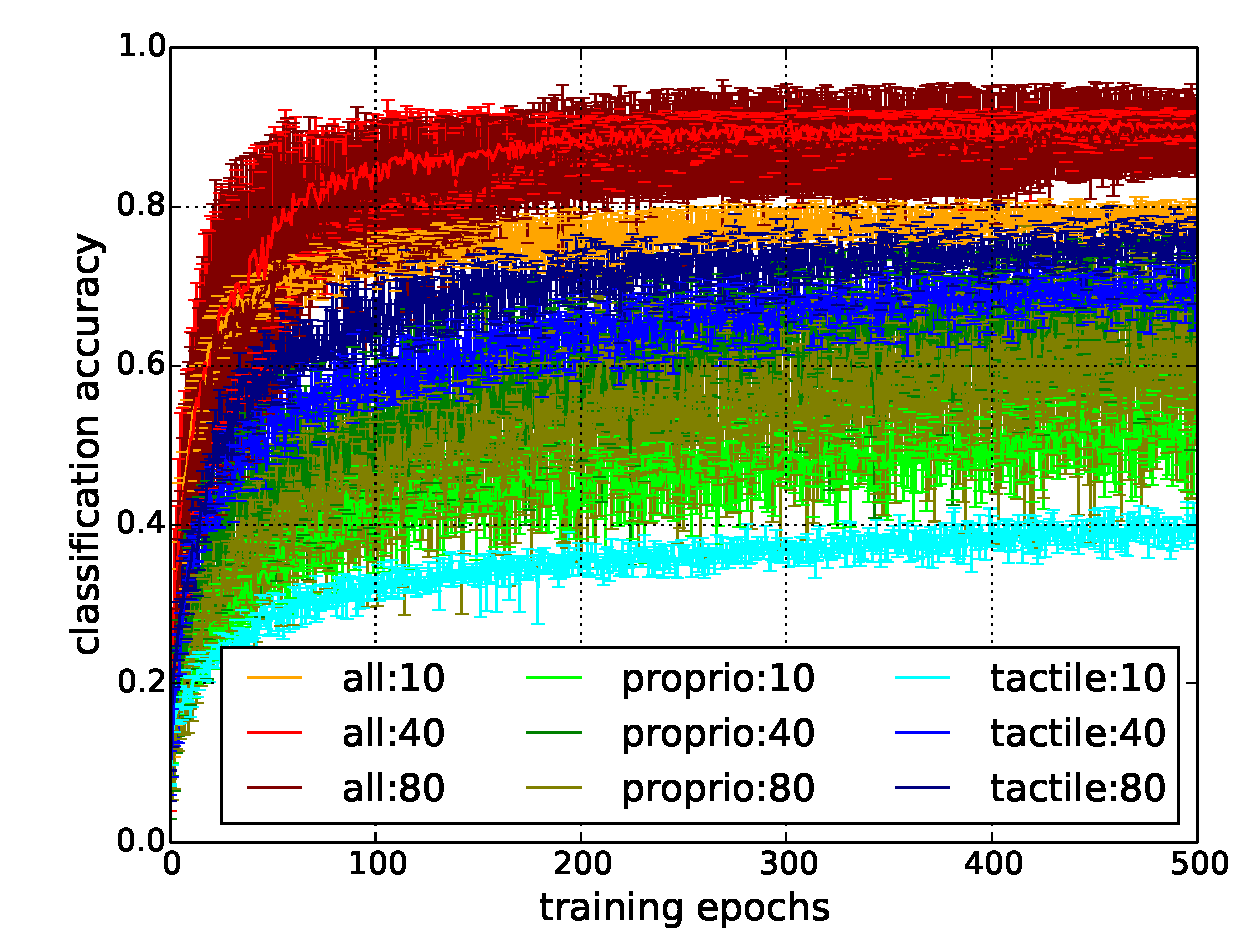
\includegraphics[width=0.9\textwidth]{cl_sen_vs_epoch}
  \caption{Evaluation of different sensor types separately (average of 10 observations, timesteps: 10, 40, 80).}
  \label{fig:sen_vs_epoch}
\end{figure}

\cref{fig:sen_vs_epoch} shows that the combination of the two types results with the highest classification accuracy, namely even with $ 10 $ simulation steps (1 second of real time) compared to $ 40 $ (4 seconds), resp. $ 80 $ (8 seconds), for only one of the sensor types. Having more time for classification ($ 4 $ or $ 8 $ seconds), the six tactile sensors are more successful than proprioceptive, however, they fail when the classification needs to be fast ($ 1 $ second). Complete classification results for all of these configurations can be found in \cref{tab:classification_results}.

Number of used sensors affects the size of the feature vector and hence also the size of the network input layer. The dimensionality of the network mattrices influence the processing time. An average epoch time out of 10 observations is shown for the two sensor types in \cref{fig:sen_time}. 

\begin{figure}[H]
  \centering
  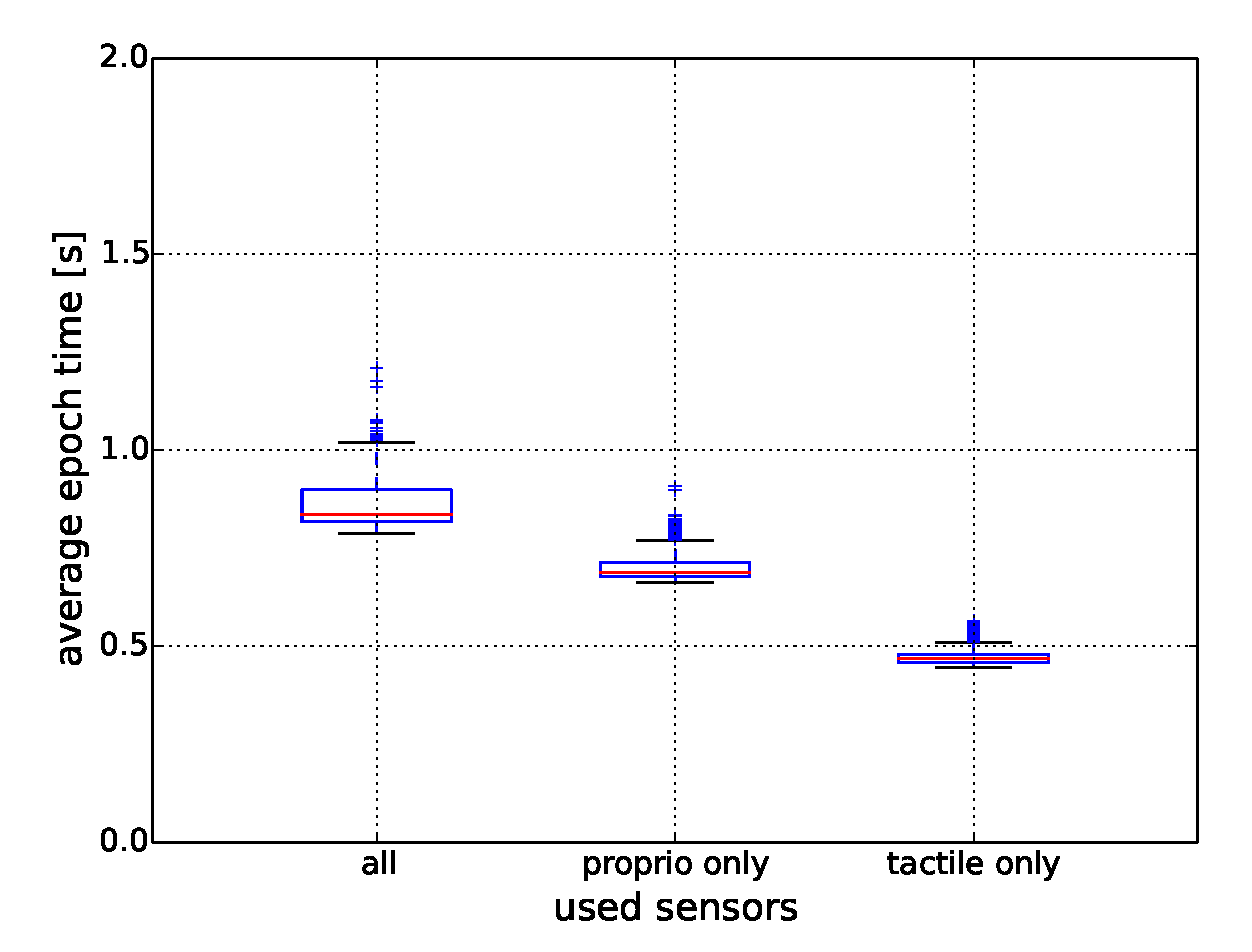
\includegraphics[width=0.8\textwidth]{cl_sen_time}
  \caption{Average epoch time for different sensor types.}
  \label{fig:sen_time}
\end{figure}

\subsection{Comparison to SOA Methods} \label{ssec:terrain_classification_vs_soa}
TODO: brief comparison to results of the vison-based method (maybe just in discussion)

\newpage
\section[Terrain Classification Using Network Pruning]{Terrain Classification Using Network Pruning} \label{sec:pa_amter}
In this section, the developed pruning algorithm (\cref{sec:network_pruning_algorithm}) is applied on the terrain classification problem (\cref{chap:terrain_classification}). The datasets containing the terrain data are listed in \cref{app:tab:generated_datasets}. On each of them, a neural network was trained, evaluated and saved (classification results in \cref{tab:classification_results}). These trained nets were used as the input of the pruning algorithm to obtain the following results.

The configurations listed in \cref{tab:configurations_for_pa} were chosen for demonstration of the PA on terrain classification:

\begin{table}[H]
\centering
\caption{Chosen configurations for PA demonstration.}
\label{tab:configurations_for_pa}
\begin{tabular}{|c|c|c|c|c|c|}
\hline
  & \textit{dataset} & \textit{\begin{tabular}[c]{@{}c@{}}ter./sig.\\  noise\end{tabular}} & \textit{timesteps} & \textit{sensors} & \textit{\begin{tabular}[c]{@{}c@{}}hidden\\ neurons\end{tabular}} \\ \hline
A & 00\_00\_40\_a    & 0/0                                                                 & 40                 & all              & 20                                                                \\ \hline
B & 00\_00\_80\_a    & 0/0                                                                 & 80                 & all              & 20                                                                \\ \hline
C & 00\_00\_40\_a    & 0/0                                                                 & 40                 & all              & 100                                                               \\ \hline
D & 03\_03\_40\_a    & 0.03/0.03                                                           & 40                 & all              & 20                                                                \\ \hline
E & 00\_00\_40\_p    & 0/0                                                                 & 40                 & proprioceptive   & 20                                                                \\ \hline
F & 00\_00\_40\_t    & 0/0                                                                 & 40                 & tactile          & 20                                                                \\ \hline
\end{tabular}
\end{table}

The result of the pruning algorithm applied on the default configuration (A) is illustrated in \cref{fig:pa_result_amter}. The required classification accuracy, number of synapses and network structure are shown with respect to the pruning step. The result was obtained by averaging $ 10 $ observations.

\begin{figure}[H]
  \centering
  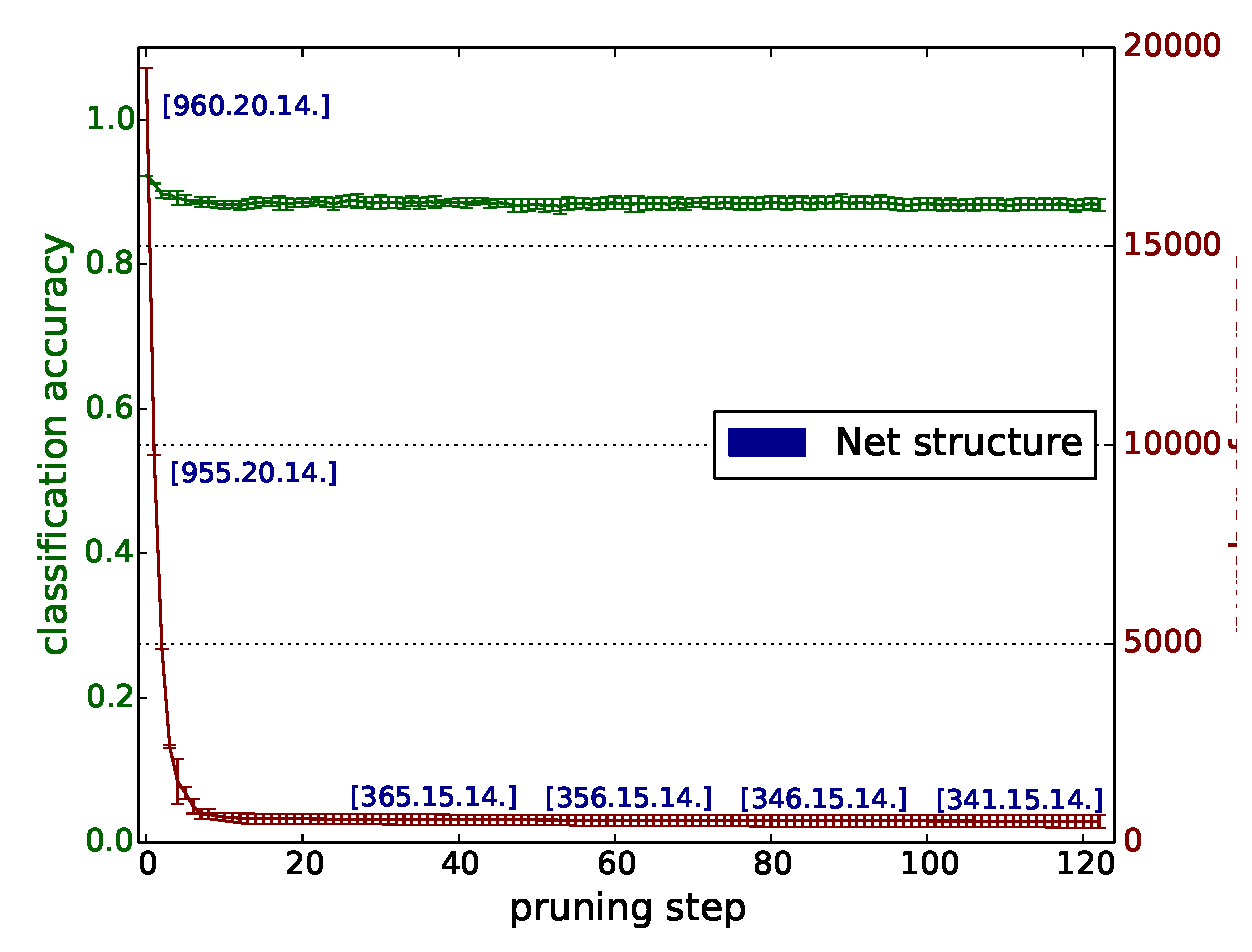
\includegraphics[width=1.0\textwidth]{pa_result_amter_nn}
  \caption{Pruning Algorithm Results on AMTER Dataset. No noise.}
  \label{fig:pa_result_amter}
\end{figure}

The number of synapses was reduced from $ 19400 $ to $ 516 $. Complete results for all the listed configurations from \cref{tab:configurations_for_pa} are presented in \cref{tab:amter_pa_results}.

\begin{table}[H]
\centering
\caption{Results of the PA on terrain datasets.}
\label{tab:amter_pa_results}
\resizebox{\textwidth}{!} {
\begin{tabular}{|c|c|c|c|c|c|c|c|}
\hline
           & \textit{\begin{tabular}[c]{@{}c@{}}required\\ accuracy\end{tabular}} & \textit{\begin{tabular}[c]{@{}c@{}}structure\\ before\end{tabular}} & \textit{\begin{tabular}[c]{@{}c@{}}synapses\\ before\end{tabular}} & \textit{\begin{tabular}[c]{@{}c@{}}structure\\ after\end{tabular}} & \textit{\begin{tabular}[c]{@{}c@{}}synapses\\ after\end{tabular}} & \textit{\begin{tabular}[c]{@{}c@{}}accuracy on\\ testing set\end{tabular}} & \textit{\begin{tabular}[c]{@{}c@{}}pruning\\ steps\end{tabular}} \\ \hline
\textbf{A} & 0.9                                                                  & {[}960, 20, 14{]}                                                   & 19400                                                              & {[}330, 16, 14{]}                                                  & 516                                                               & 0.8807                                                                     & 123                                                              \\ \hline
\textbf{A*} & 0.75                                                                  & {[}960, 20, 14{]}                                                   & 19400                                                              & {[}69, 10, 13{]}                                                  & 123                                                               & 0.6437                                                                     & 27                                                              \\ \hline
\textbf{B} & 0.9                                                                  & {[}1920, 20, 14{]}                                                  & 38680                                                              & {[}399, 16, 14{]}                                                  & 531                                                               & 0.8859                                                                     & 363                                                              \\ \hline
\textbf{C} & 0.65                                                                 & {[}960, 100, 14{]}                                                  & 97400                                                              & {[}136, 33, 14{]}                                                  & 204                                                               & 0.7384                                                                     & 28                                                               \\ \hline
\textbf{D} & 0.7                                                                  & {[}960, 20, 14{]}                                                   & 19400                                                              & {[}331, 17, 14{]}                                                  & 534                                                               & 0.6787                                                                     & 76                                                               \\ \hline
\textbf{E} & 0.65                                                                 & {[}720, 20, 14{]}                                                   & 14680                                                              & {[}116, 8, 12{]}                                                   & 182                                                               & 0.6601                                                                     & 92                                                               \\ \hline
\textbf{F} & 0.65                                                                 & {[}240, 20, 14{]}                                                   & 5080                                                               & {[}44, 16, 13{]}                                                   & 144                                                               & 0.6601                                                                     & 46                                                               \\ \hline
\end{tabular}}
\end{table}

As we can see, the network \textit{D}, trained on noisy the noisy dataset, ends with very similar results as the reference \textit{A} configuration. The structural and synaptic reduction of configuration \textit{B} (using 80 timesteps) takes more pruning steps, but also ends up with comparable results. As \textit{A}, \textit{B} requires the same accuracy, we can compare their synaptic pruning process in a graph (\cref{fig:pa_amter_synapses_90}). Additionally, configuration \textit{D} is included, as its pruning progress is also comparable.

\begin{figure}[H]
  \centering
  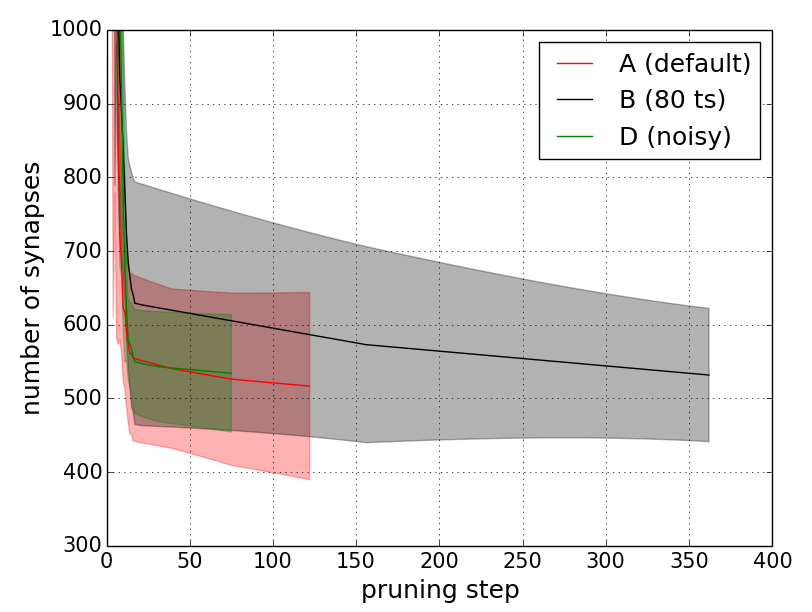
\includegraphics[width=0.9\textwidth]{pa_amter_synapses_acc90.png}
  \caption{Synaptic pruning of configurations A (reference), B (80 timesteps) and D (noisy data).}
  \label{fig:pa_amter_synapses_90}
\end{figure}

Similarly, we can compare the remaining configurations (\textit{C}, \textit{E}, and \textit{F}), as all of them requires the accuracy of $ 0.65 $ (\cref{fig:pa_amter_synapses_65}. Additionally, the \textit{A} (default) configuration is pruned with the same required accuracy as \textit{C} ($ 0.75 $) and added for comparison (liste as \textit{A*}). Ideally, \textit{A*} would end up with the same result as the huge network (\textit{C}).

Interestingly, when pruning \textit{E} and \textit{F} configurations, the PA decided to omit some of the terrains completely (see \cref{tab:amter_pa_results} and \cref{fig:pa_amter_used_neurons_65}), which is allowed since only $ 65\% $ of accuracy was required. 

\begin{figure}[H]
  \centering
  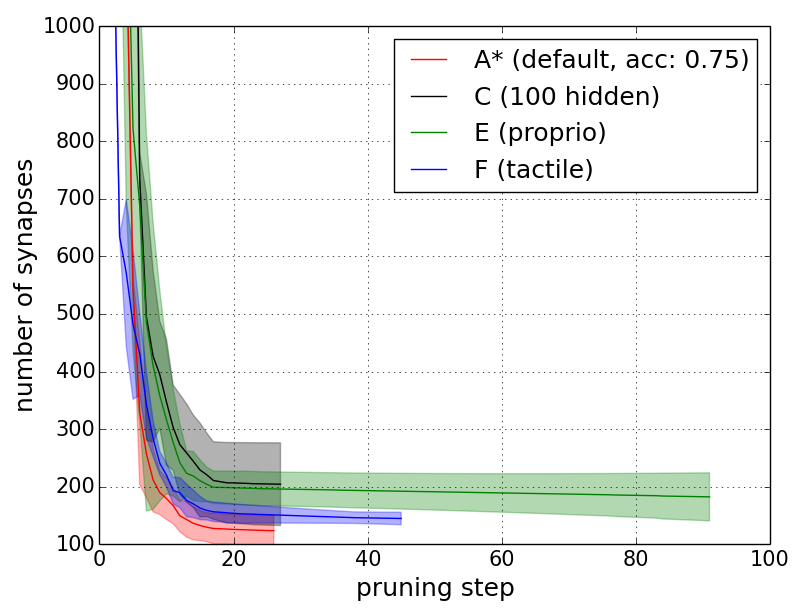
\includegraphics[width=0.9\textwidth]{pa_amter_synapses_acc65.png}
  \caption{Synaptic pruning of configurations A* (reference), C (100 hidden neurons), E (proprioceptive sensors) and F (tactile sensors).}
  \label{fig:pa_amter_synapses_65}
\end{figure}

The following \cref{fig:pa_amter_used_neurons_90} shows a relative amount of active neurons after pruning for configurations \textit{A}, \textit{B} and \textit{D}. Each configuration is also labeled by the required accuracy and the initial number of neurons per layer.

\begin{figure}[H]
  \centering
  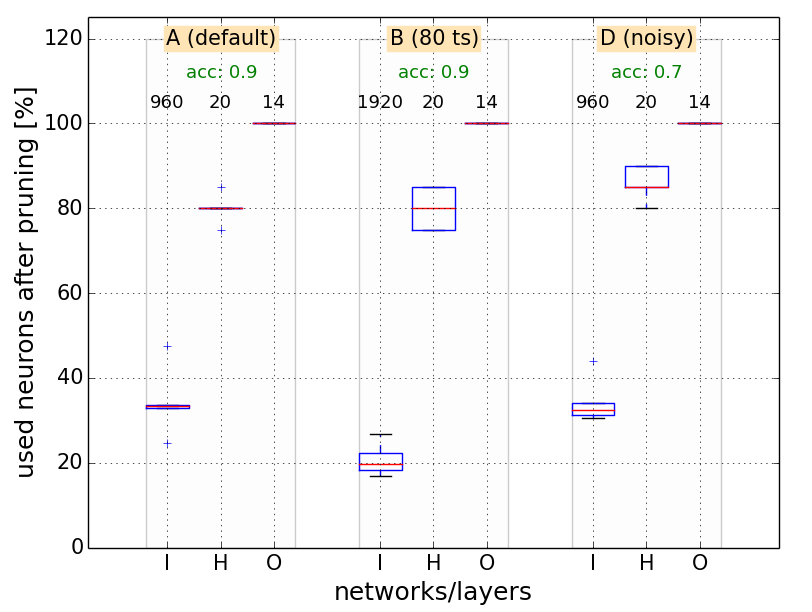
\includegraphics[width=0.8\textwidth]{pa_result_amter_used_neurons_90.png}
  \caption{Active neurons in the network after pruning [\%]: configurations A, B, D (10 observations)}
  \label{fig:pa_amter_used_neurons_90}
\end{figure}

In \cref{fig:pa_amter_used_neurons_65}, the same statistics for configurations \textit{C}, \textit{E} and \textit{F}, completed by \textit{A*}, is shown. In general, input layers are reducted the most. The results also indicate that proprioceptive sensing does not need that many hidden units compared to tactile sensing.

\begin{figure}[H]
  \centering
  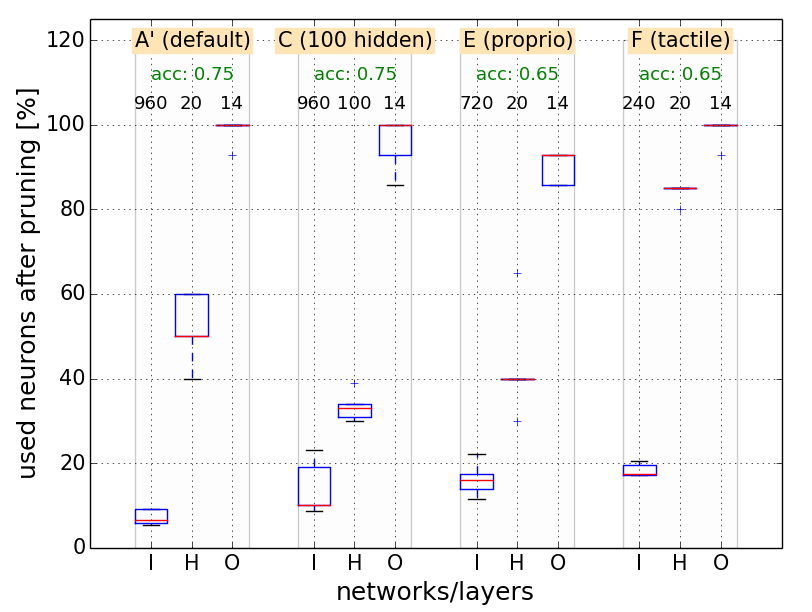
\includegraphics[width=0.8\textwidth]{pa_result_amter_used_neurons_65.png}
  \caption{Active neurons in the network after pruning [\%]: configurations A*, C, E, F (10 observations)}
  \label{fig:pa_amter_used_neurons_65}
\end{figure}

\subsection{Feature Selection for Terrain Classification} \label{ssec:pa_amter_feature_selection}
Section \ref{ssec:minimal_structure_util} presents an idea of using minimal structures for feature selection. The idea is based on tracking paths from input neurons representing individual features to output neurons (classes). This approach was applied on the minimal structure of the \textit{A} configuration from \cref{tab:amter_pa_results}, hence tha analysis is performed on a network of structure $ [330, 16, 14] $ with $ 516 $ synapses.

\cref{fig:pa_amter_n_paths_to_output} shows three sample examples (right y-axis). On the left y-axis, number of paths (see \cref{img:path_explanation}) to the output layer is counted for each feature.

\begin{figure}[H]
  \centering
  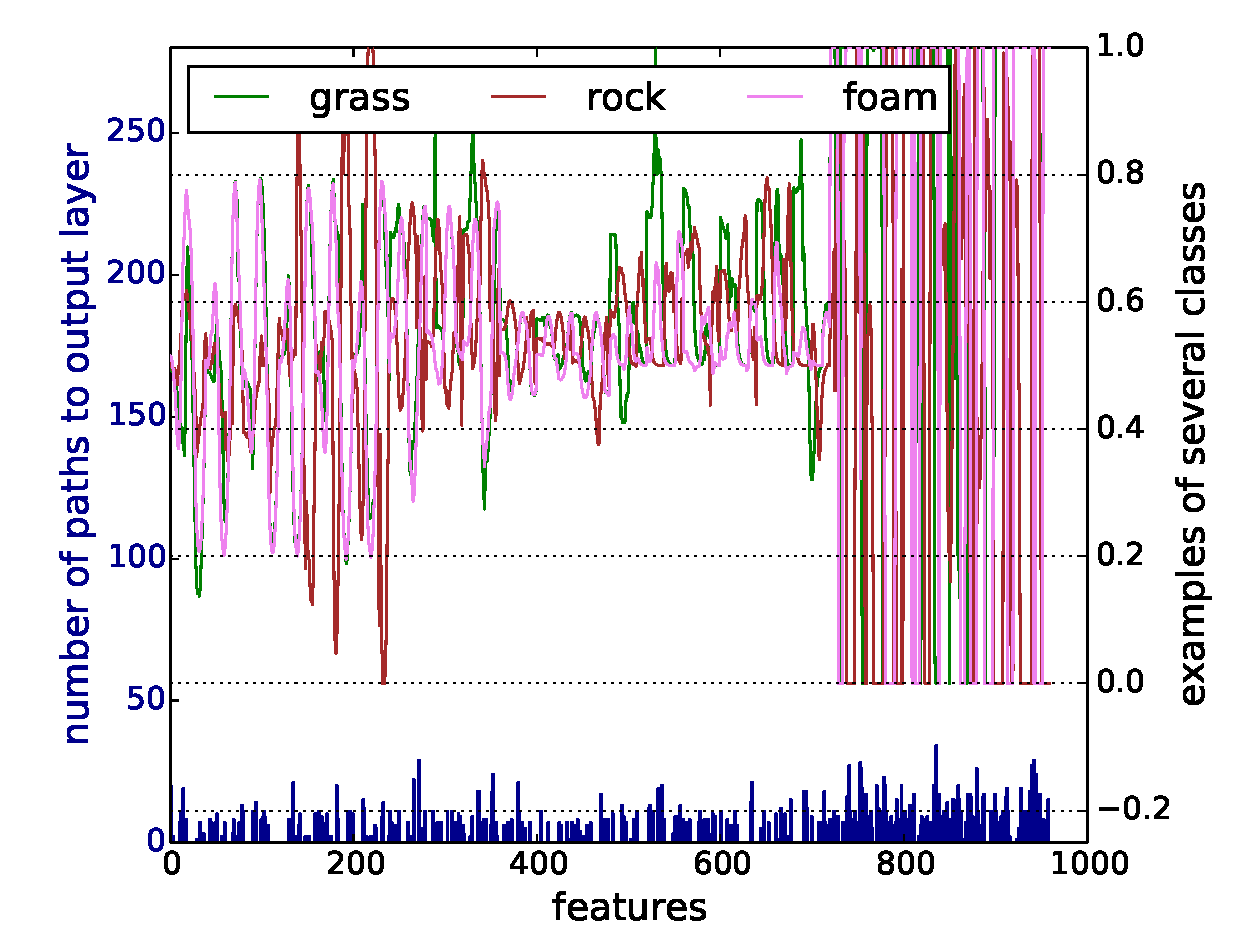
\includegraphics[width=0.8\textwidth]{fs_n_paths_to_output}
  \caption{Number of paths to the output layer for every feature of the input example.}
  \label{fig:pa_amter_n_paths_to_output}
\end{figure}

\cref{img:path_explanation} explains the meaning of a path in this context.

\begin{figure}[H]
  \centering
  \includegraphics[width=0.5\textwidth]{path_explanation.png}
  \caption{Explanation of a path from input to output layer in a minimal structure.}
  \label{img:path_explanation}
\end{figure}

Having these paths, we can distinguish features important for individual classes. In \cref{fig:pa_amter_used_features_thoraco}, the analysis is done for every feature of the Thoraco-Coxa joint angle sensors. Red dots means that the feature has a path to the corresponding class (terrain).

\begin{figure}[H]
  \centering
  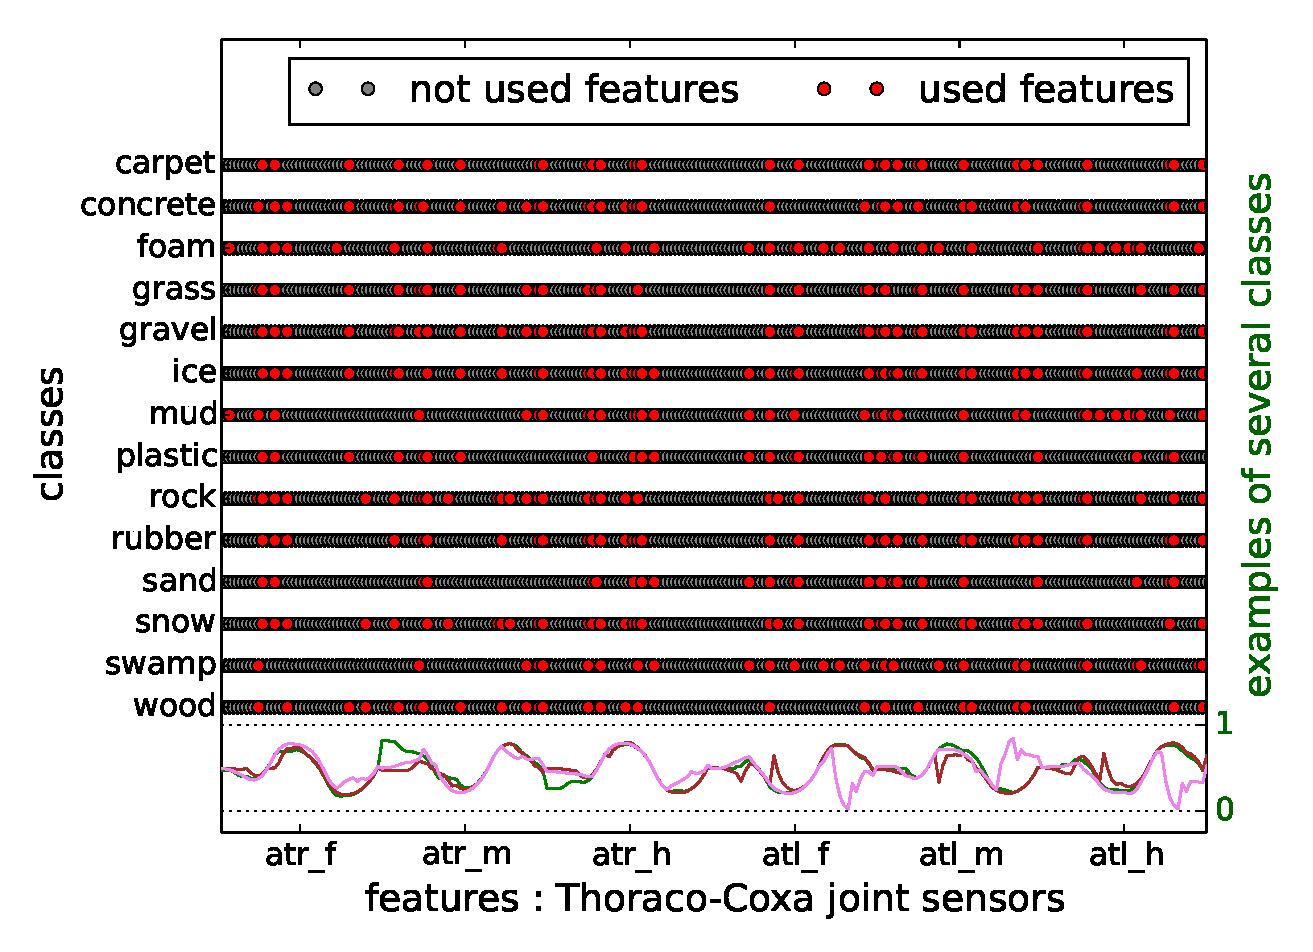
\includegraphics[width=0.75\textwidth]{fs_used_features_thoraco}
  \caption{Used features of thoraco-coxa proprioceptive sensors for individual classes.}
  \label{fig:pa_amter_used_features_thoraco}
\end{figure}

The same analysis for tactile sensors is shown in \cref{fig:pa_amter_used_features_tactile}. Similar figures for \textit{coxa} and \textit{femur} joint angle sensors can be found in \cref{app:sec:complete_feature_analysis_for_terrains}.

Using this analysis, one might find the redundant parts of the feature vector, as some of the features are unimportant for any of the classes. Moreover, we can make statements about single features based on the classes it is connected to. For instance, if a feature, belonging to the foot contact sensor on the right front leg, fires for foam and does not fire for the other classes, we might assume that this sensor is important if we want to classify foam properly.

To go even further with this analysis, also weights of the minimal network structure can be used. \cref{fig:pa_amter_io_power_tactile} shows \textit{powers}, which a single feature contributes with, to forming values on individual classes. 

\begin{figure}[H]
  \centering
  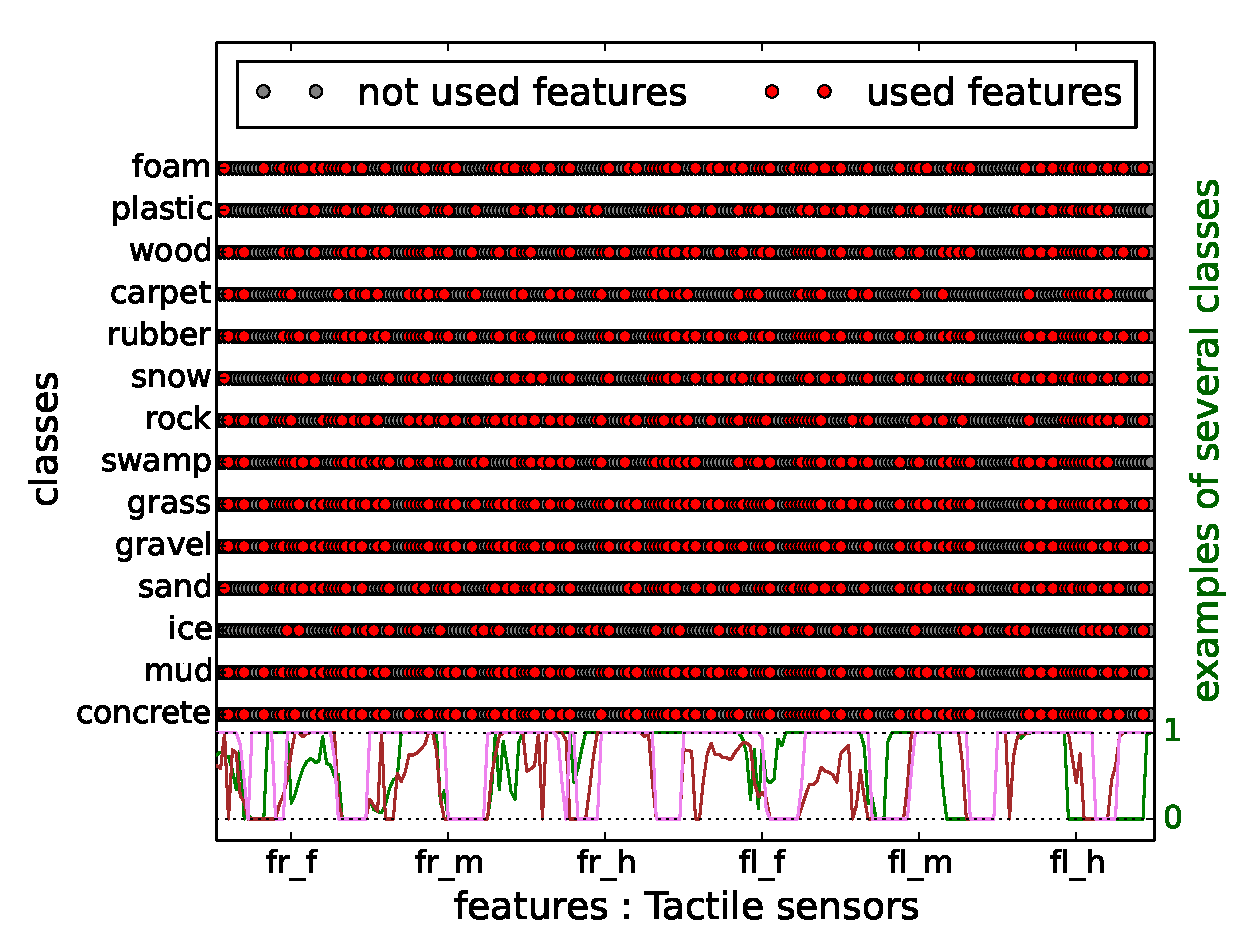
\includegraphics[width=0.75\textwidth]{fs_used_features_tactile}
  \caption{Used features of tactile sensors for individual classes.}
  \label{fig:pa_amter_used_features_tactile}
\end{figure}

The \textit{power} of feature \textit{f}, corresponding to input neuron $ i_r $, and class \textit{c}, represented by output neuron $ o_q $, is computed as given in \cref{eq:io_power}; (assuming one hidden layer).
\noindent
\begin{align} \label{eq:io_power}
power_{r,q} = \displaystyle{\sum_{k=1}^{N_{hidden}} w_{r, k} + w_{k, q}}
\end{align}

\begin{figure}[H]
  \centering
  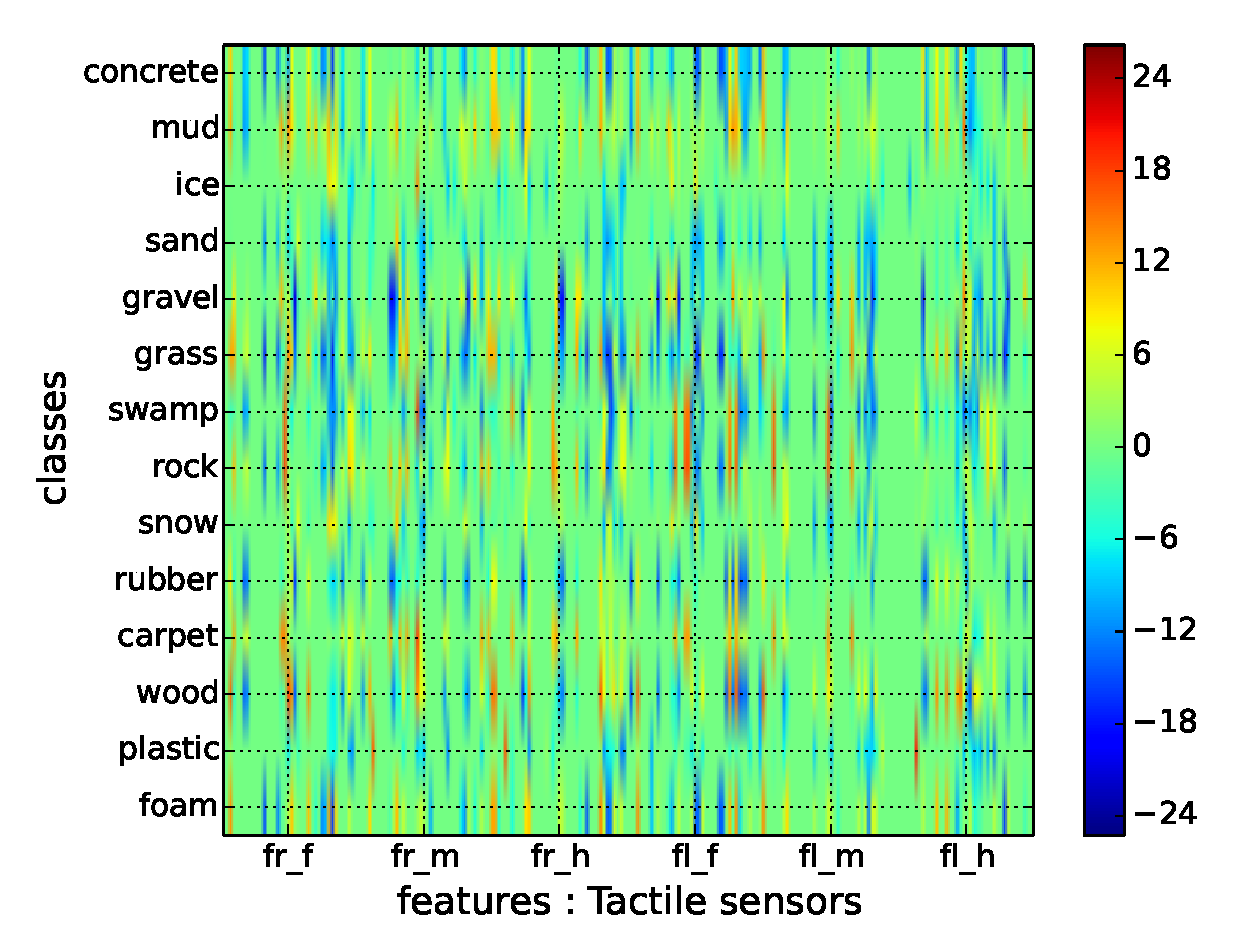
\includegraphics[width=0.75\textwidth]{fs_amter_io_power_tactile}
  \caption{Influence power of single features on classes: tactile sensors}
  \label{fig:pa_amter_io_power_tactile}
\end{figure}

Based on the results in \cref{fig:pa_amter_io_power_tactile}, besides the knowledge if a feature affects a particular class, we can also see the direction (positive/negative) and a power of this influence. For instance, we can find a feature affecting plastic or concrete positively and snow or mud negatively at the same time. 

Results for the proprioceptive sensors were generated in the same manner and can be found in \cref{app:sec:supplementary_figures_for_feature_analysis}.
